\chapter{Conception et développement du modèle d'intelligence artificielle}

\chapintro
Ce chapitre présente la partie « intelligence » du système : les modèles de vision par ordinateur qui détectent les
obstacles dans les images. Après un rappel des principes de la vision par ordinateur et de la détection d'objets,
nous présentons la famille de modèles YOLO26 et l'environnement Ultralytics. Nous décrivons ensuite la
préparation des deux jeux de données (routes réelles et piste du prototype), le développement et l'entraînement
des modèles, l'exploitation de leurs prédictions (localisation, distance, gravité, priorité) et enfin
l'évaluation de leurs performances.

% =================================================================================================
\section{Introduction à la vision par ordinateur}

\subsection{Principes de la vision par ordinateur}
La vision par ordinateur vise à extraire automatiquement de l'information d'images ou de vidéos. Pour une machine,
une image couleur est un tableau de nombres de taille $H \times W \times 3$ (hauteur, largeur, trois canaux rouge,
vert et bleu). Les méthodes classiques reposaient sur des descripteurs conçus à la main (contours, histogrammes de
gradients, couleurs). Depuis 2012, les \textbf{réseaux de neurones convolutifs} (CNN) apprennent eux-mêmes ces
descripteurs à partir d'exemples annotés : les premières couches détectent des motifs simples (bords, textures), les
couches profondes des structures de plus en plus abstraites (roues, visages, objets entiers).

Une chaîne de vision comporte généralement les étapes de la figure~\ref{fig:chaine-vision} : acquisition de
l'image, prétraitement (redimensionnement, normalisation), inférence du modèle, post-traitement des prédictions et
exploitation du résultat par l'application.

\begin{figure}[H]
\centering
\resizebox{\linewidth}{!}{%
\begin{tikzpicture}[node distance=0.55cm]
  \node[bloco,minimum width=2.4cm] (a) {Acquisition\\\scriptsize caméra, vidéo};
  \node[bloc,minimum width=2.6cm,right=of a] (b) {Prétraitement\\\scriptsize rotation, \textit{letterbox}};
  \node[blocg,minimum width=2.6cm,right=of b] (c) {Inférence\\\scriptsize réseau YOLO26};
  \node[bloc,minimum width=2.8cm,right=of c] (d) {Post-traitement\\\scriptsize seuil, coordonnées};
  \node[blocv,minimum width=2.8cm,right=of d] (e) {Exploitation\\\scriptsize distance, gravité, carte};
  \foreach \x/\y in {a/b,b/c,c/d,d/e} \draw[fleche] (\x) -- (\y);
\end{tikzpicture}}
\caption{Chaîne de traitement d'un système de vision par ordinateur}
\label{fig:chaine-vision}
\end{figure}

\subsection{Détection d'objets et segmentation d'images}
On distingue plusieurs tâches de complexité croissante :
\begin{itemize}
  \item la \textbf{classification}, qui attribue une étiquette à l'image entière (« il y a un cône ») ;
  \item la \textbf{détection d'objets}, qui localise chaque objet par une \emph{boîte englobante}
        $(x_1, y_1, x_2, y_2)$ et lui associe une classe et un score de confiance ;
  \item la \textbf{segmentation}, qui attribue une classe à chaque pixel. La segmentation d'instances distingue en
        plus les objets individuels et fournit leur contour exact (\emph{masque}).
\end{itemize}
La détection d'objets est la tâche adaptée à notre besoin : elle indique quels obstacles sont présents, où ils se
trouvent dans l'image et avec quelle confiance, tout en restant assez rapide pour le temps réel. Nous avons
cependant utilisé la segmentation à une autre étape : pour \emph{annoter} automatiquement les images de notre piste,
le modèle de segmentation SAM~2~\cite{ravi2024sam2} a produit le masque de chaque obstacle, dont la boîte englobante
se déduit directement (figure~\ref{fig:det-seg}).

\begin{figure}[H]
\centering
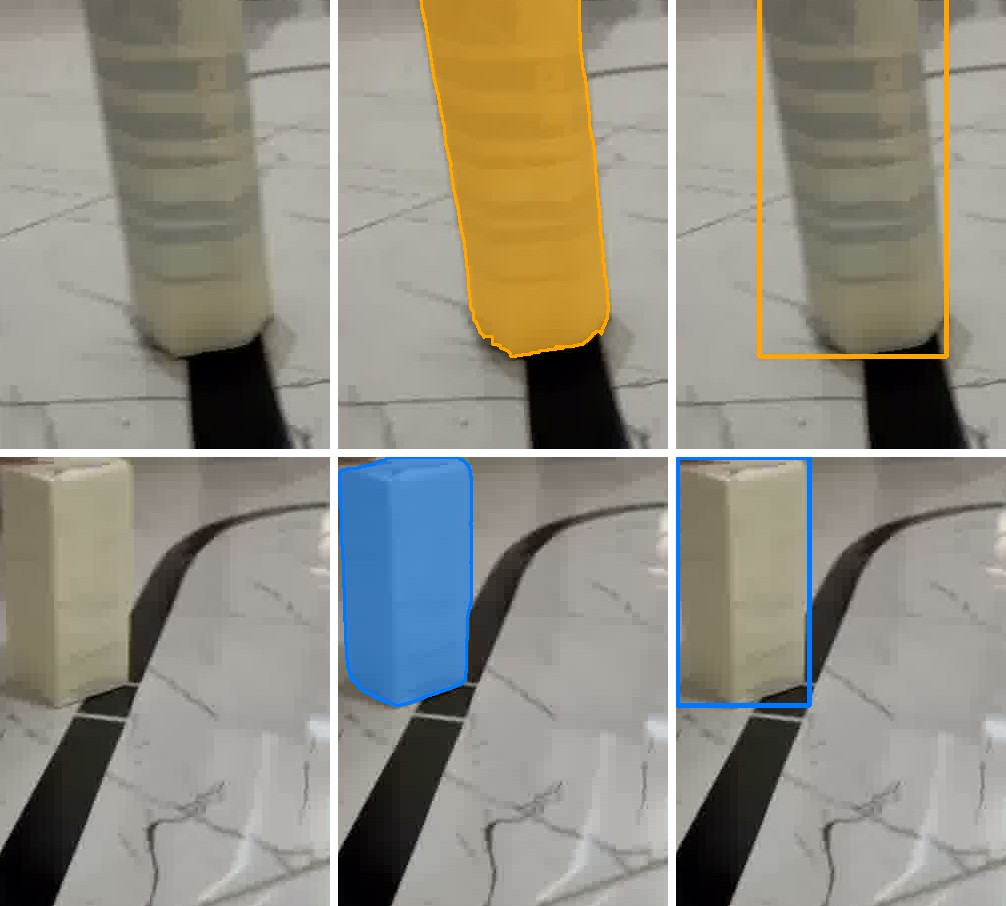
\includegraphics[width=\linewidth]{donnees/sam2_segmentation.jpg}
\caption{Image d'origine, segmentation (masque produit par SAM~2) et détection (boîte englobante déduite du
masque) pour les deux obstacles de la piste}
\label{fig:det-seg}
\end{figure}

\subsection{Application à la détection des obstacles routiers et des nids-de-poule}
Sur la route, deux familles d'obstacles doivent être reconnues. Les \textbf{usagers de la route} (piétons,
cyclistes, véhicules, animaux) sont des objets bien représentés dans les grands jeux de données publics : un
modèle préentraîné les reconnaît déjà. Les \textbf{anomalies routières} (nids-de-poule, cônes, barrières,
panneaux de chantier) sont plus spécifiques et nécessitent un apprentissage dédié. Les nids-de-poule sont les plus
difficiles : ils sont plats, de forme et de taille très variables, souvent remplis d'eau ou peu contrastés avec la
chaussée. La figure~\ref{fig:exemples-route} montre les prédictions de nos deux modèles routiers sur des images
de test.

\begin{figure}[H]
\centering
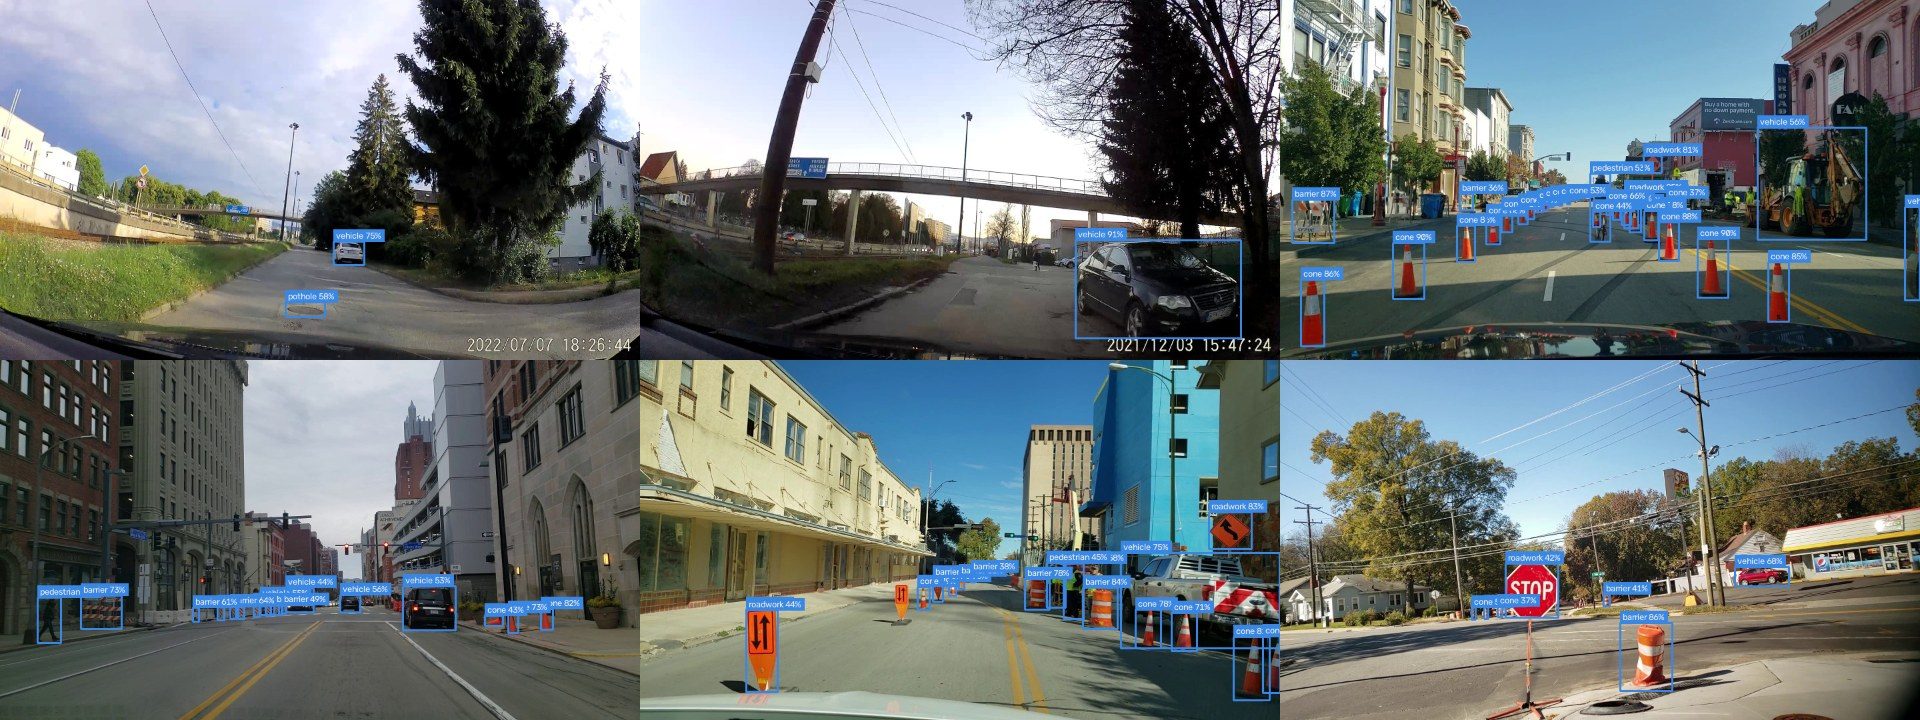
\includegraphics[width=\linewidth]{ia/reel_exemples_detection.jpg}
\caption{Détections des modèles routiers (usagers de la route et anomalies) sur des images de l'ensemble de test,
aux seuils de l'application. Les erreurs restent visibles : un nid-de-poule manqué (en haut au centre), un
panneau STOP pris pour un panneau de chantier (en bas à droite).}
\label{fig:exemples-route}
\end{figure}

% =================================================================================================
\section{Présentation des modèles YOLO26}

\subsection{Généralités sur la famille YOLO}
Les détecteurs d'objets se répartissent en deux familles. Les détecteurs \emph{à deux étapes} (R-CNN, Faster R-CNN)
proposent d'abord des régions candidates, puis les classent : ils sont précis mais lents. Les détecteurs \emph{à une
étape} prédisent directement les boîtes et les classes en une seule passe du réseau. YOLO (\textit{You Only Look
Once}), introduit par Redmon et al. en 2016~\cite{redmon2016yolo}, est le représentant le plus connu de cette
seconde famille : il découpe l'image en une grille et prédit, pour chaque cellule, des boîtes et des probabilités
de classes.

Depuis, la famille a beaucoup évolué (tableau~\ref{tab:yolo}) : ancres et prédiction multi-échelle (YOLOv3),
augmentation \textit{mosaic} (YOLOv4~\cite{bochkovskiy2020yolov4}), têtes sans ancres (YOLOv8), entraînement sans
NMS (YOLOv10~\cite{wang2024yolov10}) et, avec YOLO26, une architecture pensée pour le déploiement sur processeurs
et équipements embarqués~\cite{ultralytics26}.

\begin{table}[H]
\centering\small
\caption{Quelques étapes de l'évolution de la famille YOLO}
\label{tab:yolo}
\begin{tabular}{lll}
\toprule
\textbf{Version} & \textbf{Année} & \textbf{Apport principal} \\
\midrule
YOLO (v1)   & 2016 & Détection en une seule passe sur une grille \\
YOLOv3      & 2018 & Prédictions à trois échelles, ancres \\
YOLOv4 / v5 & 2020 & Augmentation \textit{mosaic}, écosystème PyTorch (Ultralytics) \\
YOLOv8      & 2023 & Tête sans ancres, API unifiée (détection, segmentation, pose) \\
YOLOv10     & 2024 & Affectation un-à-un : inférence sans NMS \\
YOLO11      & 2024 & Blocs C3k2 et attention C2PSA \\
YOLO26      & 2025 & Inférence de bout en bout sans NMS, suppression de la DFL, optimisé CPU / embarqué \\
\bottomrule
\end{tabular}
\end{table}

\subsection{Présentation de YOLO26 et de son architecture}
YOLO26 est la génération de détecteurs publiée par Ultralytics en 2025~\cite{ultralytics26}. Elle est déclinée en
cinq tailles : \emph{nano} (n), \emph{small} (s), \emph{medium} (m), \emph{large} (l) et \emph{extra-large} (x). Comme
ses prédécesseurs, le réseau comporte trois parties (figure~\ref{fig:yolo26}) :
\begin{itemize}
  \item un \textbf{backbone} (extracteur de caractéristiques) convolutif qui réduit progressivement la résolution
        et produit des cartes de caractéristiques à plusieurs échelles (P3, P4, P5, soit 1/8, 1/16 et 1/32 de
        l'image) ;
  \item un \textbf{neck} de type FPN/PAN~\cite{lin2017fpn,liu2018panet} qui combine ces échelles, pour détecter à la fois
        les petits objets lointains et les grands objets proches ;
  \item une \textbf{tête de détection} qui prédit, pour chaque position, la boîte et les scores de classes.
\end{itemize}
Ses principales nouveautés visent le déploiement : la tête est \textbf{de bout en bout} (affectation un-à-un) et
produit directement au plus 300 détections finales, \textbf{sans post-traitement NMS} ; la \textit{Distribution Focal
Loss} (DFL) est supprimée, ce qui simplifie l'export ; l'entraînement utilise une pondération progressive des pertes
(ProgLoss) et une affectation des étiquettes favorable aux petits objets (STAL). Exporté en ONNX, le modèle produit
un unique tenseur de sortie de taille $1 \times 300 \times 6$ : pour chaque détection, $(x_1, y_1, x_2, y_2)$, le
score et la classe. Notre modèle du prototype (YOLO26n, deux classes) compte 2,39 millions de paramètres pour
5,4 GFLOPs.

\begin{figure}[H]
\centering
\resizebox{\linewidth}{!}{%
\begin{tikzpicture}[node distance=0.3cm and 0.5cm,
  feat/.style={draw=bleufst,thick,fill=bleufst!12,minimum width=1.25cm,align=center,font=\scriptsize,rounded corners=2pt}]
  \node[bloco,minimum width=2.1cm,minimum height=2.6cm] (in) {Image\\640$\times$640$\times$3\\\scriptsize(\textit{letterbox})};
  % backbone
  \node[feat,minimum height=2.4cm,right=0.7cm of in] (b1) {Conv\\stride 2};
  \node[feat,minimum height=2.1cm,right=0.25cm of b1] (b2) {Conv\\+ C3k2};
  \node[feat,minimum height=1.8cm,right=0.25cm of b2] (b3) {C3k2\\P3/8};
  \node[feat,minimum height=1.4cm,right=0.25cm of b3] (b4) {C3k2\\P4/16};
  \node[feat,minimum height=1.05cm,right=0.25cm of b4] (b5) {SPPF\\C2PSA\\P5/32};
  \begin{scope}[on background layer]
    \node[zone,fill=bleufst!4,fit=(b1)(b5),label={[font=\bfseries\small]above:Backbone}] (bb) {};
  \end{scope}
  % neck
  \node[feat,draw=vertfst!80!black,fill=vertfst!15,minimum height=1.05cm,right=1.0cm of b5,yshift=1.25cm] (n5) {P5};
  \node[feat,draw=vertfst!80!black,fill=vertfst!15,minimum height=1.05cm,below=0.25cm of n5] (n4) {P4};
  \node[feat,draw=vertfst!80!black,fill=vertfst!15,minimum height=1.05cm,below=0.25cm of n4] (n3) {P3};
  \node[font=\scriptsize,align=center,right=0.1cm of n4] (fpn) {FPN $\downarrow$\\PAN $\uparrow$};
  \begin{scope}[on background layer]
    \node[zone,fill=vertfst!5,fit=(n5)(n3)(fpn),label={[font=\bfseries\small]above:Neck}] (nk) {};
  \end{scope}
  \draw[fleche] (b3.east) to[out=0,in=180] (n3.west);
  \draw[fleche] (b4.east) to[out=0,in=180] (n4.west);
  \draw[fleche] (b5.east) to[out=0,in=180] (n5.west);
  % head
  \node[bloc,draw=orangefst,fill=orangefst!12,minimum width=3.3cm,minimum height=2.6cm,right=0.9cm of nk]
       (head) {Tête de bout en bout\\(un-à-un, sans DFL)\\\scriptsize boîtes + classes\\\scriptsize sans NMS};
  \draw[fleche] (nk) -- (head);
  \node[bloc,minimum width=2.6cm,minimum height=2.6cm,right=0.7cm of head] (out) {Sortie\\$1 \times 300 \times 6$\\\scriptsize $x_1,y_1,x_2,y_2$,\\\scriptsize score, classe};
  \draw[fleche] (in) -- (bb); \draw[fleche] (head) -- (out);
\end{tikzpicture}}
\caption{Architecture simplifiée d'un détecteur YOLO26 : backbone, neck multi-échelle et tête de bout en bout
sans NMS}
\label{fig:yolo26}
\end{figure}

Le choix des variantes résulte d'un compromis entre précision et vitesse, l'inférence se faisant sur le processeur
de l'ordinateur : la variante \textbf{nano} pour les usagers de la route et pour le prototype, la variante
\textbf{small}, un peu plus lourde, pour les anomalies routières, plus difficiles à reconnaître.

\subsection{Utilisation des poids préentraînés sur COCO}
Entraîner un détecteur à partir de zéro demande des centaines de milliers d'images annotées. Nous utilisons
l'\textbf{apprentissage par transfert} : les modèles partent des poids publiés par Ultralytics, préentraînés sur
COCO~\cite{lin2014coco} (118\,287 images d'entraînement, 80 classes d'objets courants). Le backbone sait déjà
extraire des caractéristiques visuelles générales ; l'affinage (\textit{fine-tuning}) adapte surtout la tête aux
nouvelles classes (figure~\ref{fig:transfert}).

Pour les usagers de la route, aucun réentraînement n'est nécessaire : les classes COCO \textit{person},
\textit{bicycle}, \textit{car}, \textit{bus}, \textit{truck}, \textit{dog}, etc. sont directement regroupées en quatre
catégories utiles au véhicule (tableau~\ref{tab:classes-users}).

\begin{figure}[H]
\centering
\resizebox{0.95\linewidth}{!}{%
\begin{tikzpicture}[node distance=0.5cm and 0.8cm]
  \node[blocg,minimum width=3.2cm] (coco) {YOLO26 préentraîné\\COCO (80 classes)};
  \node[bloc,minimum width=3.4cm,above right=0.25cm and 1.2cm of coco] (u) {Usagers de la route\\\scriptsize regroupement de classes COCO};
  \node[bloco,minimum width=3.4cm,right=1.2cm of coco] (h) {Affinage sur 7\,894 images\\\scriptsize anomalies routières (YOLO26s)};
  \node[blocv,minimum width=3.4cm,below right=0.25cm and 1.2cm of coco] (t) {Affinage sur notre piste\\\scriptsize colonne / boîte (YOLO26n)};
  \draw[fleche] (coco) -- node[note,above,sloped] {sans réentraînement} (u.west);
  \draw[fleche] (coco) -- (h); \draw[fleche] (coco) -- (t.west);
  \node[bloc,minimum width=2.6cm,right=0.8cm of h] (on) {Export\\ONNX};
  \draw[fleche] (u.east) -- (on); \draw[fleche] (h) -- (on); \draw[fleche] (t.east) -- (on);
\end{tikzpicture}}
\caption{Apprentissage par transfert à partir des poids COCO}
\label{fig:transfert}
\end{figure}

\subsection{Environnement Ultralytics}
La bibliothèque Python \textbf{Ultralytics}~\cite{ultralytics26} fournit les modèles YOLO26 et toute la chaîne de
travail : chargement des jeux de données décrits par un fichier \texttt{data.yaml}, entraînement avec augmentation de
données, validation (précision, rappel, mAP, courbes et matrice de confusion), prédiction et export vers de
nombreux formats (ONNX, TensorRT, TFLite…). L'entraînement a été réalisé dans un \textbf{conteneur Docker} basé sur
l'image officielle \texttt{ultralytics/ultralytics} (Ultralytics 8.4.184, PyTorch avec CUDA), complétée par
JupyterLab, ce qui garantit un environnement identique d'une machine à l'autre. Les notebooks
\texttt{train\_road\_obstacles.ipynb} et \texttt{train\_toy\_obstacles.ipynb} s'exécutent sur ce noyau et utilisent le
GPU de l'ordinateur (NVIDIA GeForce GTX 1650 Ti, 4 Go). La figure~\ref{fig:workflow} résume le flux de travail.

\begin{figure}[H]
\centering
\resizebox{\linewidth}{!}{%
\begin{tikzpicture}[node distance=0.5cm]
  \node[bloco,minimum width=2.6cm] (d) {Données\\\scriptsize images + étiquettes};
  \node[bloc,minimum width=2.4cm,right=of d] (y) {\texttt{data.yaml}\\\scriptsize classes, splits};
  \node[blocg,minimum width=2.6cm,right=of y] (tr) {\texttt{model.train()}\\\scriptsize GPU, augmentation};
  \node[blocg,minimum width=2.6cm,right=of tr] (va) {\texttt{model.val()}\\\scriptsize test : P, R, mAP};
  \node[blocg,minimum width=2.6cm,right=of va] (ex) {\texttt{model.export()}\\\scriptsize ONNX};
  \node[blocv,minimum width=2.6cm,right=of ex] (ap) {\app\\\scriptsize ONNX Runtime};
  \foreach \a/\b in {d/y,y/tr,tr/va,va/ex,ex/ap} \draw[fleche] (\a) -- (\b);
  \begin{scope}[on background layer]
    \node[zone,fill=fond,fit=(y)(ex),label={[font=\scriptsize\bfseries]above:Notebook Jupyter — conteneur Docker Ultralytics}] {};
  \end{scope}
\end{tikzpicture}}
\caption{Flux de travail avec Ultralytics, de la préparation des données à l'intégration}
\label{fig:workflow}
\end{figure}

\subsection{Adaptation du modèle aux besoins du projet}
Les besoins du projet ont conduit à trois modèles complémentaires (tableau~\ref{tab:modeles}). En environnement
réel, deux modèles s'exécutent en parallèle sur chaque image et leurs détections sont fusionnées : l'un apporte la
connaissance générale de COCO sur les usagers de la route, l'autre la connaissance spécialisée des anomalies. Pour le
prototype, un modèle nano dédié reconnaît les deux obstacles de la piste. Les classes de chaque modèle sont
traduites vers un vocabulaire commun à l'application (\texttt{pedestrian}, \texttt{vehicle}, \texttt{pothole},
\texttt{cone}, \texttt{box}…), auquel sont associés les poids de danger utilisés pour la gravité.

\begin{table}[H]
\centering\small
\caption{Les trois modèles du projet}
\label{tab:modeles}
\begin{tabularx}{\linewidth}{l l l X}
\toprule
\textbf{Modèle} & \textbf{Variante} & \textbf{Entraînement} & \textbf{Classes détectées} \\
\midrule
Usagers de la route & YOLO26n & préentraîné COCO & piéton, cycliste, véhicule, animal \\
Anomalies routières & YOLO26s & affiné 8 h, 36 époques & nid-de-poule, cône, barrière, panneau de chantier \\
Obstacles du prototype & YOLO26n & affiné 30 min, 73 époques & colonne, boîte \\
\bottomrule
\end{tabularx}
\end{table}

% =================================================================================================
\section{Préparation des données}

\subsection{Présentation des données réelles}
Le modèle d'anomalies routières a été entraîné sur la réunion de deux jeux de données publics d'images de caméras
embarquées :
\begin{itemize}
  \item \textbf{Potholes under challenging conditions}~\cite{bucko2022potholes} (Bučko et al., \textit{Sensors},
        2022, licence CC BY 4.0) : des images de nids-de-poule extraites de vidéos de conduite en Slovaquie, dans
        des conditions difficiles (pluie, ombres, nuit, chaussée mouillée) ;
  \item \textbf{ROADWork}~\cite{ghosh2025roadwork} (Ghosh et al., ICCV 2025, Carnegie Mellon University, licence
        ODC-By 1.0) : des images de zones de travaux dans plusieurs villes, avec des cônes, des barrières et des
        panneaux de signalisation temporaire.
\end{itemize}
Au total, \textbf{7\,894 images} réelles ont été retenues. Les annotations d'origine ont été converties au format
YOLO et leurs nombreuses sous-catégories regroupées en quatre classes. La figure~\ref{fig:donnees-reelles} montre
des images d'entraînement et la répartition des étiquettes.

\begin{figure}[H]
\centering
\begin{subfigure}[b]{0.52\linewidth}\centering
  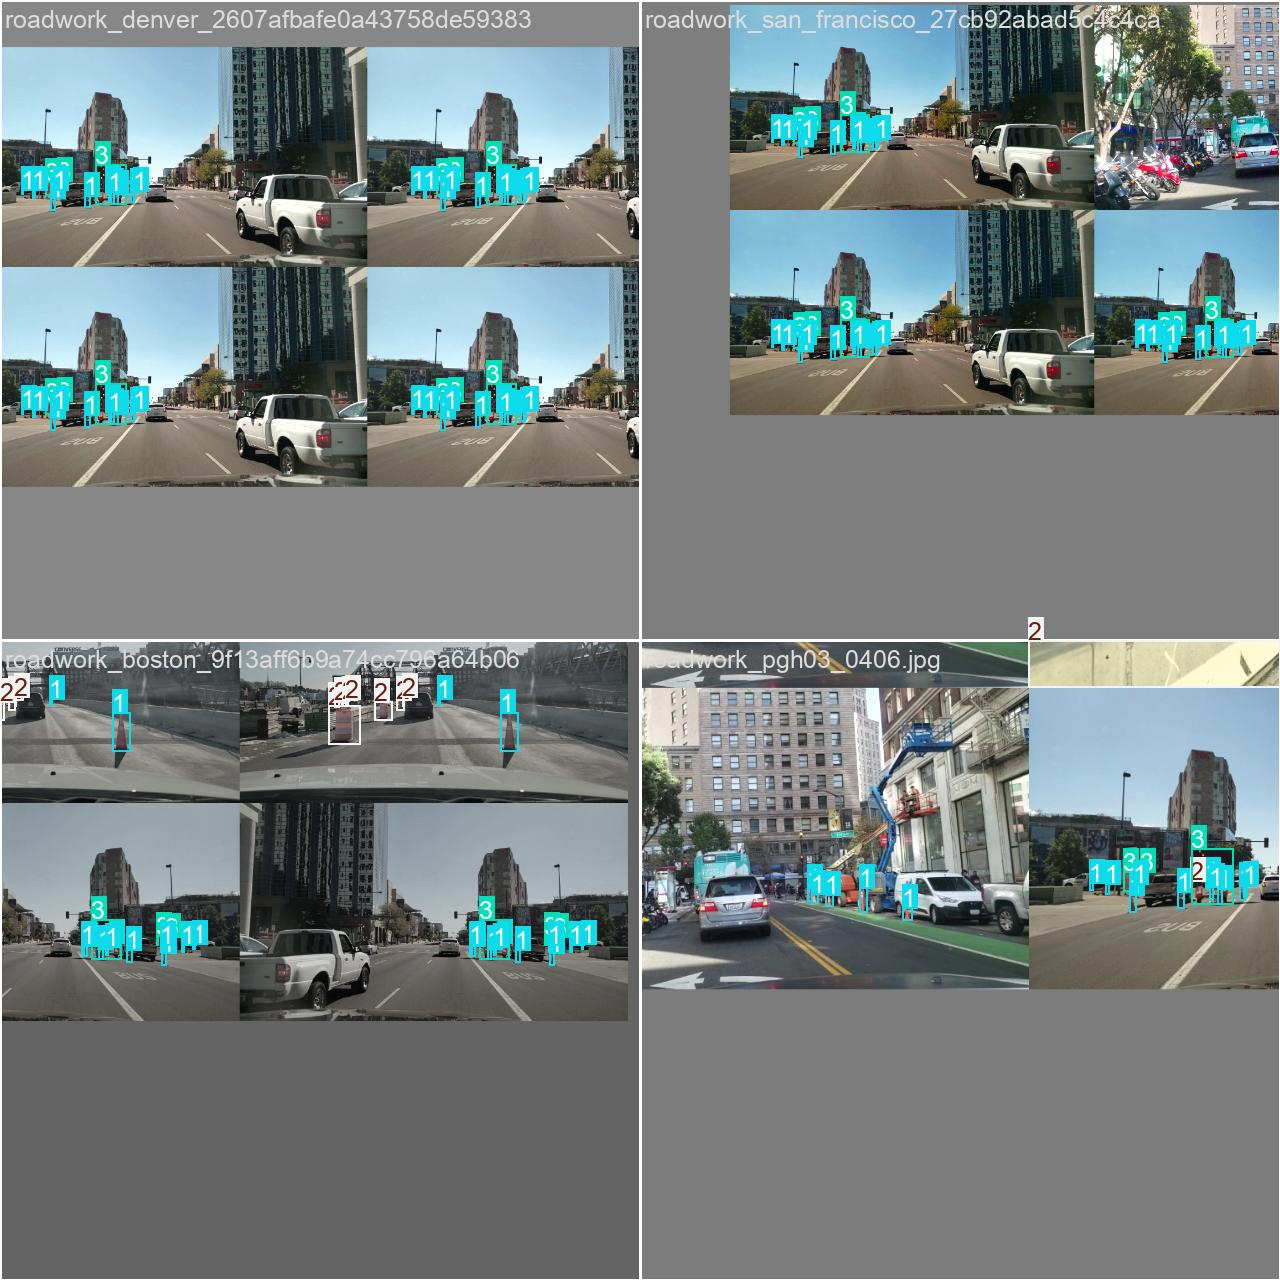
\includegraphics[width=\linewidth]{ia/reel_train_batch.jpg}
  \caption{Lot d'entraînement (mosaïques augmentées)}
\end{subfigure}\hfill
\begin{subfigure}[b]{0.45\linewidth}\centering
  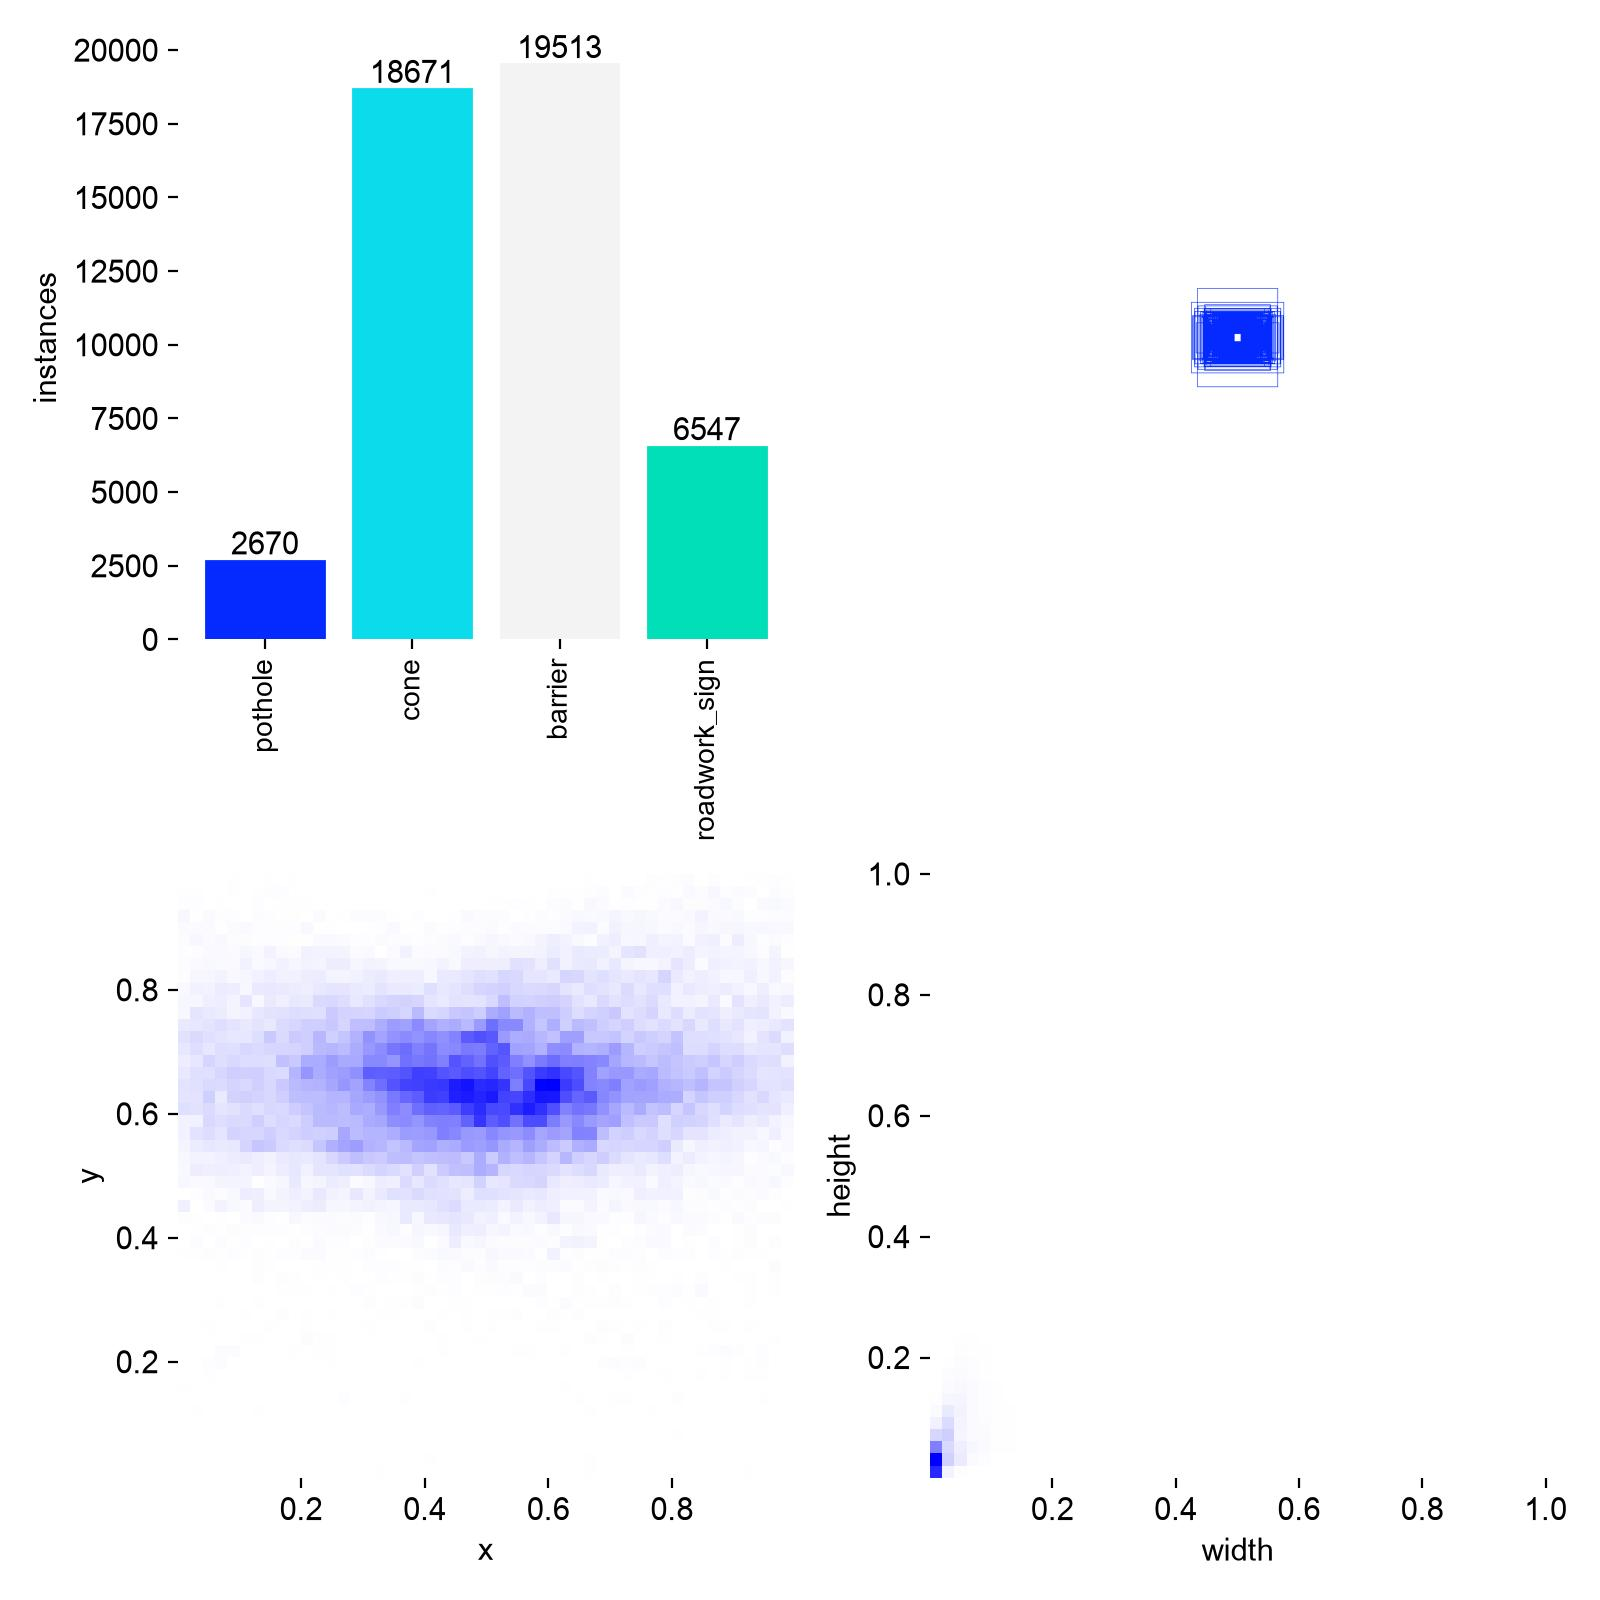
\includegraphics[width=\linewidth]{ia/reel_labels.jpg}
  \caption{Statistiques des étiquettes}
\end{subfigure}
\caption{Données réelles : exemples d'images d'entraînement et distribution des annotations}
\label{fig:donnees-reelles}
\end{figure}

Les vidéos qui alimentent la caméra embarquée de CAR-01 dans l'application proviennent de sources libres
(Wikimedia Commons, licences CC BY, CC BY-SA ou domaine public) et des images de test du jeu Potholes : elles ne
servent qu'à la démonstration, jamais à l'entraînement.

\subsection{Présentation des données du prototype}
Aucun jeu de données public ne contient notre piste et nos obstacles. Nous avons donc constitué le nôtre : une
vidéo filmée à hauteur de voiture en suivant le ruban, dont nous avons extrait \textbf{249 images}
(832\,$\times$\,464 pixels). La vidéo contient des passages devant la colonne, devant la boîte (sous plusieurs
faces, dont celle portant le logo) et des portions de piste vide (figure~\ref{fig:donnees-proto}). Une photo de la
piste vue de dessus et une photo de chaque obstacle ont complété ces images pour définir précisément les classes.

\begin{figure}[H]
\centering
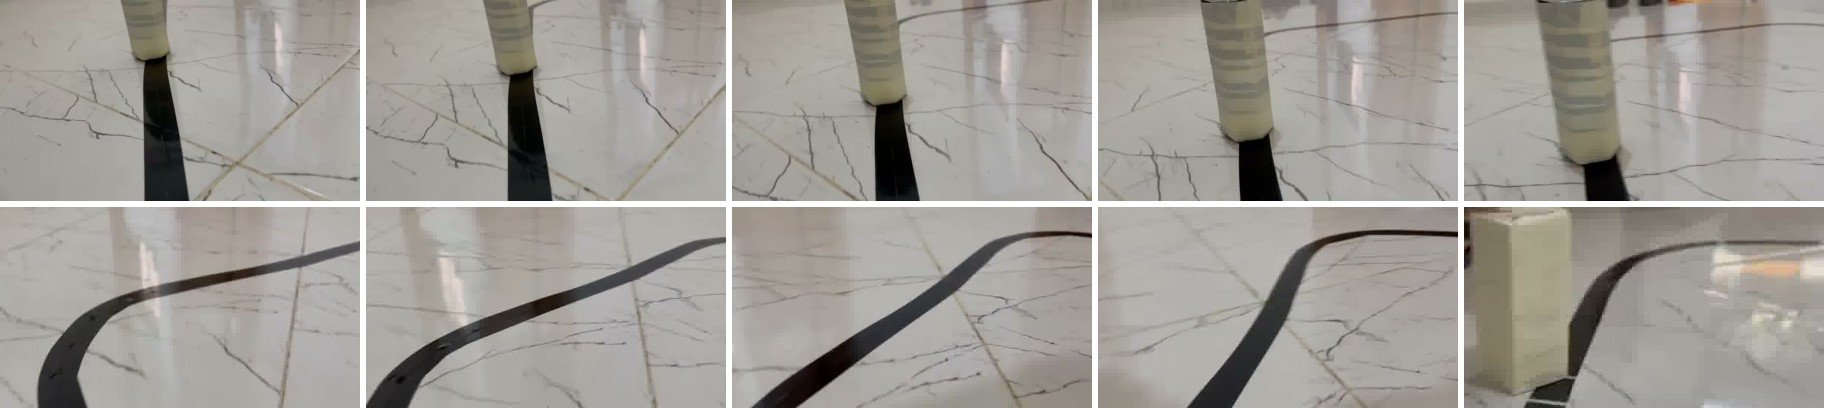
\includegraphics[width=\linewidth]{donnees/toy_frames.jpg}
\caption{Données du prototype : images extraites de la vidéo (passage devant la colonne, piste vide, boîte)}
\label{fig:donnees-proto}
\end{figure}

\subsection{Organisation et annotation des images}
Les deux jeux de données suivent l'organisation standard d'Ultralytics : un dossier \texttt{images/} et un dossier
\texttt{labels/}, chacun divisé en \texttt{train}, \texttt{val} et \texttt{test}. Chaque image possède un fichier texte
contenant une ligne par objet :
\begin{center}
\texttt{<classe> <x\_centre> <y\_centre> <largeur> <hauteur>}
\end{center}
où les coordonnées sont normalisées entre 0 et 1. Une image sans objet a un fichier vide : elle sert d'exemple
négatif (« rien à détecter ici »).

Pour les données du prototype, l'annotation manuelle de chaque image aurait été longue. Nous avons utilisé le
\textbf{suivi vidéo de SAM~2} (\textit{Segment Anything Model 2})~\cite{ravi2024sam2} : pour chaque séquence où un
obstacle est visible, un seul clic sur l'obstacle dans une image de référence suffit ; SAM~2 propage ensuite le
masque dans toute la séquence, en avant et en arrière (figure~\ref{fig:sam2}). Un filtre élimine les pixels très
sombres pour ne pas inclure le ruban noir sous la colonne. Les boîtes sont déduites des masques et \textbf{toutes ont
été vérifiées visuellement} sur des planches de contrôle. On obtient 248 images annotées (une image floue a été
écartée) contenant 141 boîtes.

\begin{figure}[H]
\centering
\resizebox{\linewidth}{!}{%
\begin{tikzpicture}[node distance=0.5cm]
  \node[bloco,minimum width=2.6cm] (v) {Vidéo\\\scriptsize 249 images};
  \node[bloc,minimum width=2.8cm,right=of v] (c) {1 clic par séquence\\\scriptsize image de référence};
  \node[blocg,minimum width=2.8cm,right=of c] (s) {Suivi SAM~2\\\scriptsize masques sur la séquence};
  \node[bloc,minimum width=2.6cm,right=of s] (f) {Filtre\\\scriptsize pixels du ruban};
  \node[bloc,minimum width=2.6cm,right=of f] (b) {Boîtes YOLO\\\scriptsize + masques};
  \node[blocv,minimum width=2.6cm,right=of b] (r) {Vérification\\\scriptsize planches visuelles};
  \foreach \x/\y in {v/c,c/s,s/f,f/b,b/r} \draw[fleche] (\x) -- (\y);
\end{tikzpicture}}

\vspace{0.3cm}
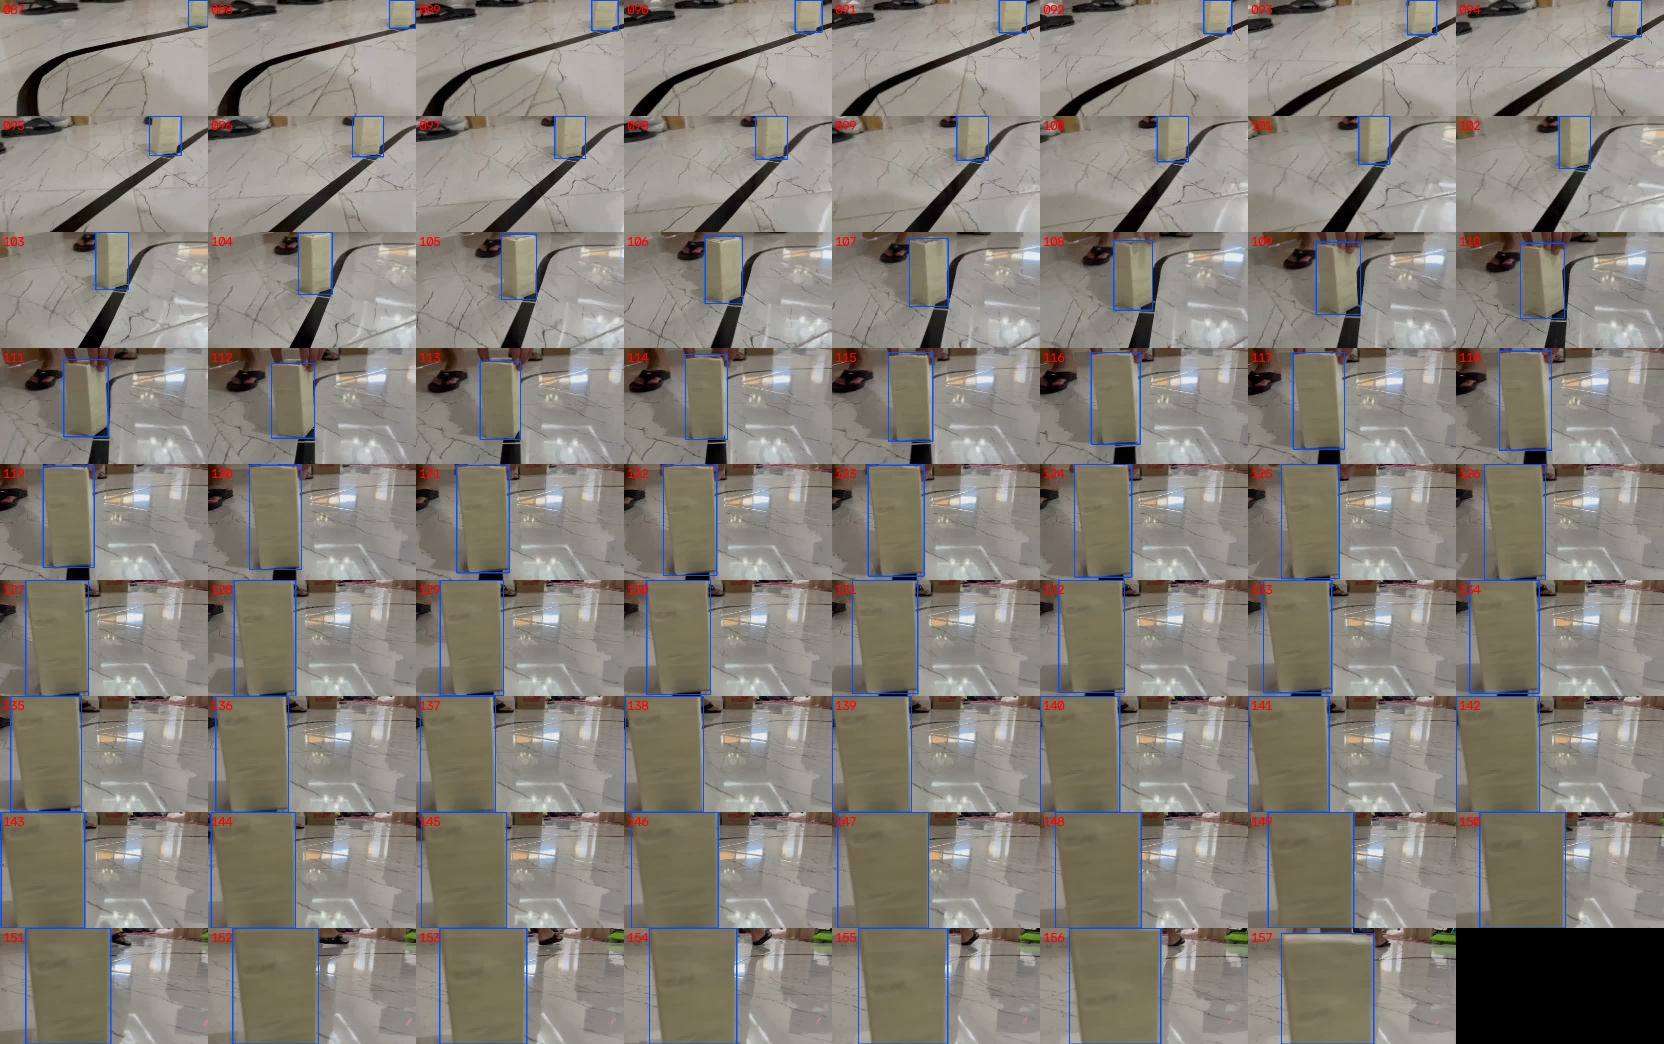
\includegraphics[width=0.95\linewidth]{donnees/toy_sam2_suivi.jpg}
\caption{Annotation automatique par suivi vidéo avec SAM~2 : chaîne de traitement et planche de contrôle d'une
séquence de la boîte}
\label{fig:sam2}
\end{figure}

\subsection{Définition des classes à reconnaître}
Les classes ont été définies en fonction de l'usage : chacune doit correspondre à une réaction différente du
véhicule ou à un niveau de danger différent (tableaux~\ref{tab:classes-users} et~\ref{tab:classes-hazards}).

\begin{table}[H]
\centering\small
\caption{Classes du modèle des usagers de la route (regroupement des classes COCO)}
\label{tab:classes-users}
\begin{tabular}{ll}
\toprule
\textbf{Classe de l'application} & \textbf{Classes COCO regroupées} \\
\midrule
\texttt{pedestrian} (piéton) & person \\
\texttt{cyclist} (cycliste) & bicycle \\
\texttt{vehicle} (véhicule) & car, motorcycle, bus, truck, train \\
\texttt{animal} & dog, cat, horse, cow, sheep, bird \\
\bottomrule
\end{tabular}
\end{table}

\begin{table}[H]
\centering\small
\caption{Classes des modèles entraînés}
\label{tab:classes-hazards}
\begin{tabularx}{\linewidth}{l l X}
\toprule
\textbf{Modèle} & \textbf{Classe} & \textbf{Contenu} \\
\midrule
Anomalies & \texttt{pothole} & nids-de-poule \\
          & \texttt{cone} & cônes et balises tubulaires \\
          & \texttt{barrier} & fûts, barricades, barrières, clôtures, panneaux verticaux \\
          & \texttt{roadwork\_sign} & panneaux de chantier, flèches lumineuses, panneaux à messages \\
\midrule
Prototype & \texttt{column} & colonne rayée à sommet noir \\
          & \texttt{box} & boîte de couleur crème (logo rouge sur une face) \\
\bottomrule
\end{tabularx}
\end{table}

\subsection{Prétraitement et augmentation des données}
Toutes les images sont redimensionnées en conservant leurs proportions et complétées par des bandes
(\textit{letterbox}) jusqu'à la taille d'entrée du réseau : 640\,$\times$\,640 pour le modèle routier,
320\,$\times$\,320 pour le prototype, résolution proche de celle de l'ESP32-CAM.

Pendant l'entraînement, Ultralytics applique des augmentations aléatoires qui multiplient la variété des
exemples : assemblage de quatre images en mosaïque (désactivé pendant les 10 dernières époques), variations de
teinte, de saturation et de luminosité, translations, changements d'échelle ($\pm 50\,\%$) et symétries
horizontales.

Pour le prototype, deux augmentations spécifiques ont été développées :
\begin{itemize}
  \item \textbf{l'aspect ESP32-CAM} : la vidéo a été filmée avec un téléphone en 16:9, alors que l'ESP32-CAM
        fournit des images 4:3 de moindre qualité. 60\,\% des images d'entraînement sont donc converties en images
        « style ESP32-CAM » : recadrage aléatoire au format 4:3, réduction à 320\,$\times$\,240, flou, dominante de
        couleur, bruit et forte compression JPEG ; les boîtes sont recalculées et un obstacle coupé à plus de 60\,\%
        par le recadrage est écarté (figure~\ref{fig:augmentation}a) ;
  \item \textbf{le copier-coller}~\cite{ghiasi2021copypaste} : les obstacles, découpés grâce à leur masque SAM~2, sont
        collés sur des images de piste vide, à de nouvelles positions et distances (plus grands lorsqu'ils sont
        proches de la caméra), avec ajustement de la luminosité. 400 images supplémentaires sont ainsi créées, avec des
        boîtes exactes (figure~\ref{fig:augmentation}b).
\end{itemize}

\begin{figure}[H]
\centering
\begin{subfigure}[b]{0.49\linewidth}\centering
  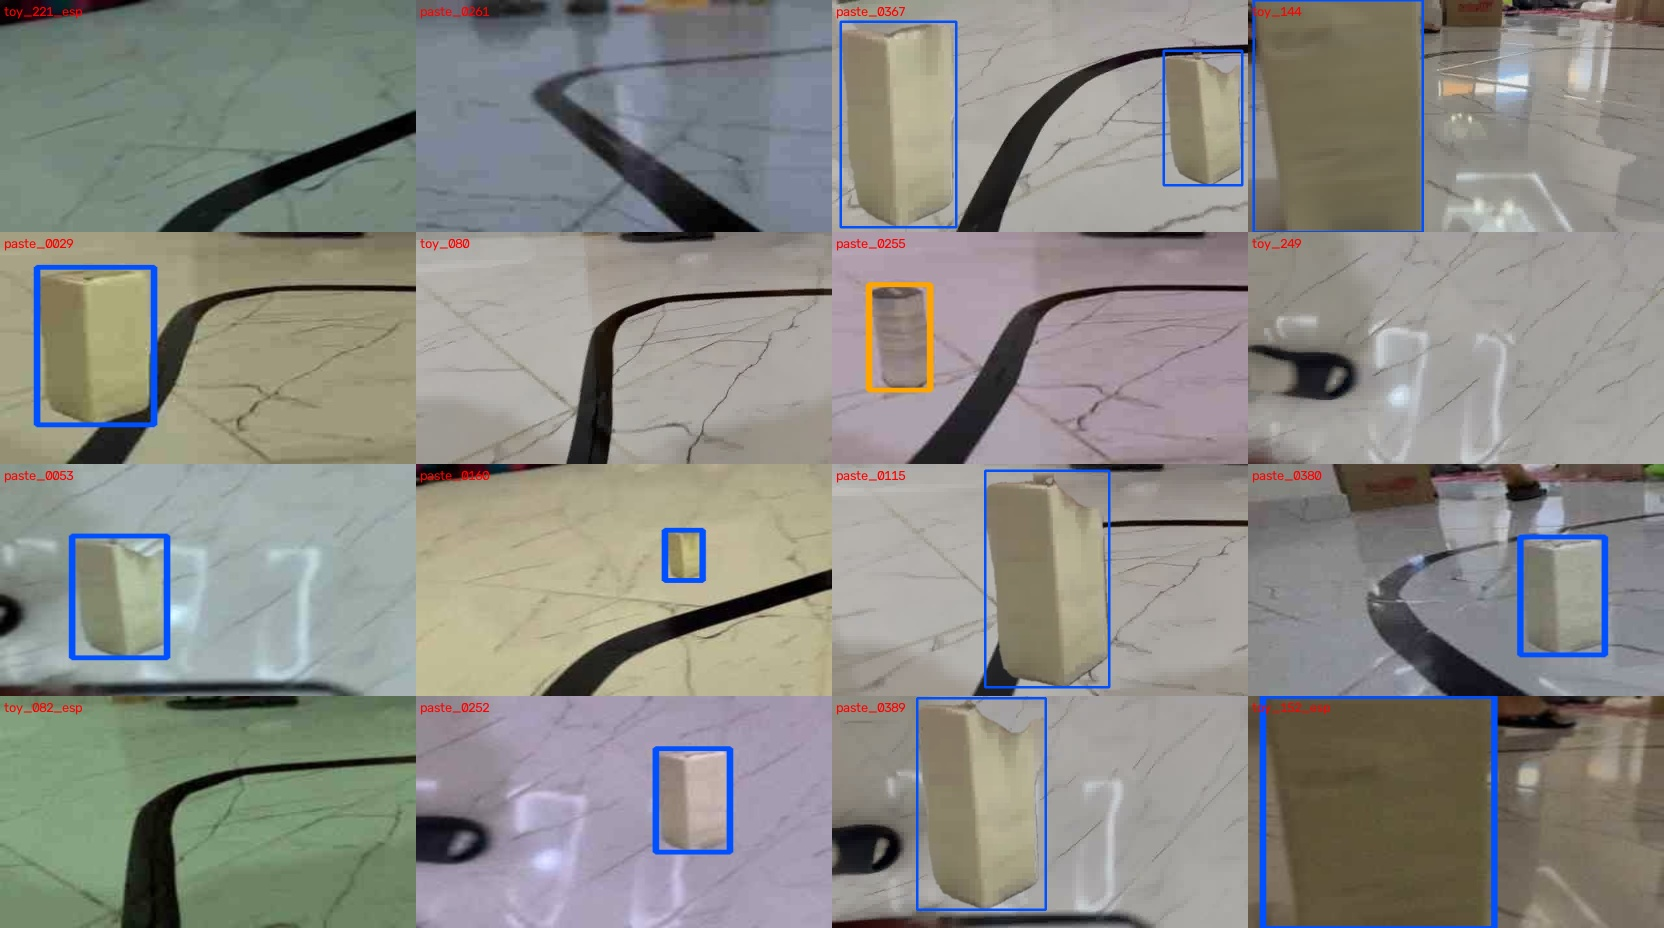
\includegraphics[width=\linewidth]{donnees/toy_esp32_look.jpg}
  \caption{Images converties au style ESP32-CAM}
\end{subfigure}\hfill
\begin{subfigure}[b]{0.49\linewidth}\centering
  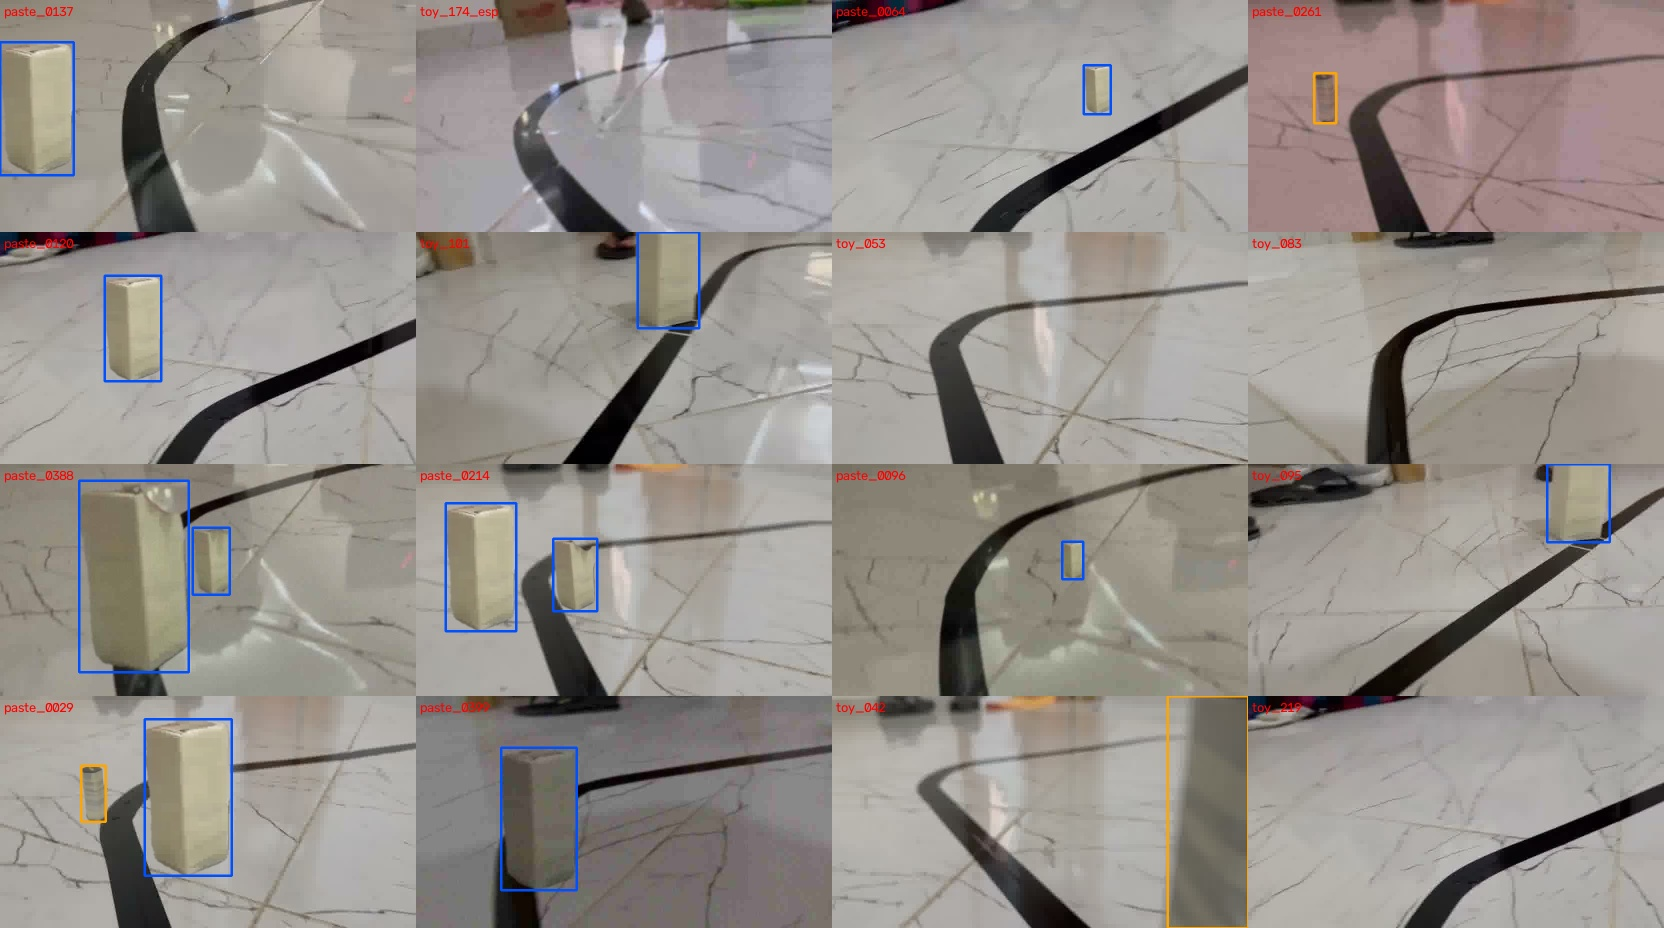
\includegraphics[width=\linewidth]{donnees/toy_train_images.jpg}
  \caption{Images d'entraînement, dont copier-coller}
\end{subfigure}
\caption{Augmentations spécifiques au prototype}
\label{fig:augmentation}
\end{figure}

\subsection{Division des données en ensembles d'entraînement, de validation et de test}
Les données sont réparties en trois ensembles : l'\textbf{entraînement} sert à ajuster les poids, la
\textbf{validation} à suivre l'apprentissage et à choisir les réglages, et le \textbf{test}, jamais utilisé avant
l'évaluation finale, à mesurer les performances.

Une précaution est essentielle avec des images extraites de vidéos : deux images voisines sont presque
identiques. Une répartition aléatoire placerait des quasi-doublons à la fois en entraînement et en test et
gonflerait artificiellement les résultats. Nous avons donc découpé \textbf{dans le temps} :
\begin{itemize}
  \item pour les nids-de-poule, chaque trajet est divisé en 80\,/\,10\,/\,10\,\% avec un intervalle de séparation ;
        pour ROADWork, la répartition géographique officielle est conservée (validation et test proviennent de lieux
        absents de l'entraînement) ;
  \item pour le prototype, chaque séquence de la vidéo est découpée en blocs temporels : un bloc pour la
        validation, un autre pour le test, le reste pour l'entraînement, avec des images d'intervalle exclues
        (figure~\ref{fig:split}).
\end{itemize}

\begin{figure}[H]
\centering
\begin{tikzpicture}[x=1.45cm,y=1cm]
  \foreach \a/\b/\c/\t in {0/3.4/bleufst/Entraînement,3.8/4.8/orangefst/Validation,5.2/6.2/vertfst!80!black/Test,
                           6.6/10/bleufst/Entraînement}
    {\fill[\c!35,draw=\c] (\a,0) rectangle (\b,0.6); \node[font=\scriptsize] at ({(\a+\b)/2},0.3) {\t};}
  \foreach \a/\b in {3.4/3.8,4.8/5.2,6.2/6.6} \filldraw[fill=gris!25,draw=gris] (\a,0) rectangle (\b,0.6);
  \draw[fleche] (0,-0.25) -- (10.2,-0.25) node[right,font=\scriptsize] {temps};
  \node[font=\scriptsize,gris] at (5,-0.6) {(intervalles gris : images exclues, pour séparer les ensembles)};
\end{tikzpicture}
\caption{Découpage temporel d'une séquence vidéo du prototype}
\label{fig:split}
\end{figure}

\begin{table}[H]
\centering\small
\caption{Répartition des données}
\label{tab:split}
\begin{tabular}{lrrr}
\toprule
\textbf{Ensemble} & \textbf{Entraînement} & \textbf{Validation} & \textbf{Test} \\
\midrule
Anomalies routières (images réelles) & 6\,324 & 755 & 815 \\
\quad objets annotés dans le test & & & 5\,105 \\
Prototype — images réelles de la vidéo & 169 & 26 & 26 \\
\quad + images style ESP32-CAM & 96 & — & 26 \\
\quad + images par copier-coller & 400 & — & — \\
\bottomrule
\end{tabular}
\end{table}

Le test du prototype comprend 26 images réelles (15 obstacles, 11 images de piste vide) et leurs 26 équivalents
convertis au style ESP32-CAM 320\,$\times$\,240, qui constituent un second ensemble de test plus proche des
conditions réelles.

% =================================================================================================
\section{Développement des deux modèles}

\subsection{Modèle destiné aux données réelles}
Le modèle d'anomalies routières est un YOLO26s affiné à partir des poids COCO sur les 6\,324 images
d'entraînement. Il est associé au modèle COCO des usagers de la route : les deux sont décrits dans un \emph{profil}
(\texttt{models/real\_road.json}) qui indique, pour chacun, le fichier ONNX, la taille d'entrée, le seuil de
confiance et la correspondance des classes. Les deux modèles s'exécutent en parallèle sur chaque image de la
caméra embarquée.

\subsection{Modèle destiné au prototype}
Le modèle du prototype est un YOLO26n affiné sur les 665 images d'entraînement (169 réelles, 96 au style
ESP32-CAM et 400 par copier-coller). La variante nano et l'entrée 320\,$\times$\,320 permettent une analyse en
temps réel du flux de la caméra sur le processeur. Son profil (\texttt{models/proto\_toy.json}) est chargé
automatiquement lorsque l'application est en mode Prototype.

\subsection{Configuration des modèles et des poids préentraînés}
Le tableau~\ref{tab:hyper} résume la configuration d'entraînement. La carte graphique (GTX 1650 Ti, 4 Go) a imposé
deux adaptations : la précision mixte (AMP) étant instable sur ce modèle de GPU, Ultralytics l'a désactivée et
l'entraînement s'est fait en 32 bits ; la taille de lot a été réduite à 4 images pour le modèle \emph{small} afin
de tenir dans la mémoire. Pour le modèle routier, la durée a été fixée par un budget de temps de 8 heures (paramètre
\texttt{time}) plutôt que par un nombre d'époques.

\begin{table}[H]
\centering\small
\caption{Configuration d'entraînement des deux modèles}
\label{tab:hyper}
\begin{tabular}{lll}
\toprule
\textbf{Paramètre} & \textbf{Anomalies routières} & \textbf{Prototype} \\
\midrule
Modèle de départ & \texttt{yolo26s.pt} (COCO) & \texttt{yolo26n.pt} (COCO) \\
Taille d'entrée & 640\,$\times$\,640 & 320\,$\times$\,320 \\
Taille de lot & 4 & 16 \\
Durée & budget de 8 h (36 époques) & 80 époques max. (arrêt à 73) \\
Arrêt anticipé (\textit{patience}) & 100 époques & 30 époques \\
Taux d'apprentissage & 0,01, décroissance en cosinus & 0,01, décroissance en cosinus \\
Mosaïque & oui, désactivée les 10 dernières époques & idem \\
Précision de calcul & FP32 (AMP désactivée) & FP32 \\
Matériel & GTX 1650 Ti (4 Go) & GTX 1650 Ti (4 Go) \\
Durée réelle & 8,0 h & 30 min \\
\bottomrule
\end{tabular}
\end{table}

\subsection{Procédure d'entraînement et de validation}
À chaque époque, le modèle parcourt l'ensemble d'entraînement par lots ; pour chaque lot, il calcule une fonction
de perte qui combine une perte de localisation (écart entre boîtes prédites et réelles, à base d'IoU) et une perte
de classification, puis met à jour ses poids par descente de gradient. À la fin de chaque époque, il est évalué sur
l'ensemble de validation et les meilleurs poids sont conservés (\texttt{best.pt}). Les notebooks affichent la
progression en temps réel ; un notebook de suivi (\texttt{monitor\_training.ipynb}) permet de consulter les courbes
pendant un entraînement de longue durée.

La figure~\ref{fig:courbes} présente les courbes d'apprentissage des deux modèles. Pour le modèle routier, les
pertes diminuent régulièrement et le mAP de validation progresse encore à la fin du budget de 8 heures, ce qui
indique qu'un entraînement plus long améliorerait encore le modèle. Pour le prototype, les métriques de validation
atteignent rapidement leur maximum et l'arrêt anticipé intervient à la 73\textsuperscript{e} époque.

\begin{figure}[H]
\centering
\begin{subfigure}[b]{\linewidth}\centering
  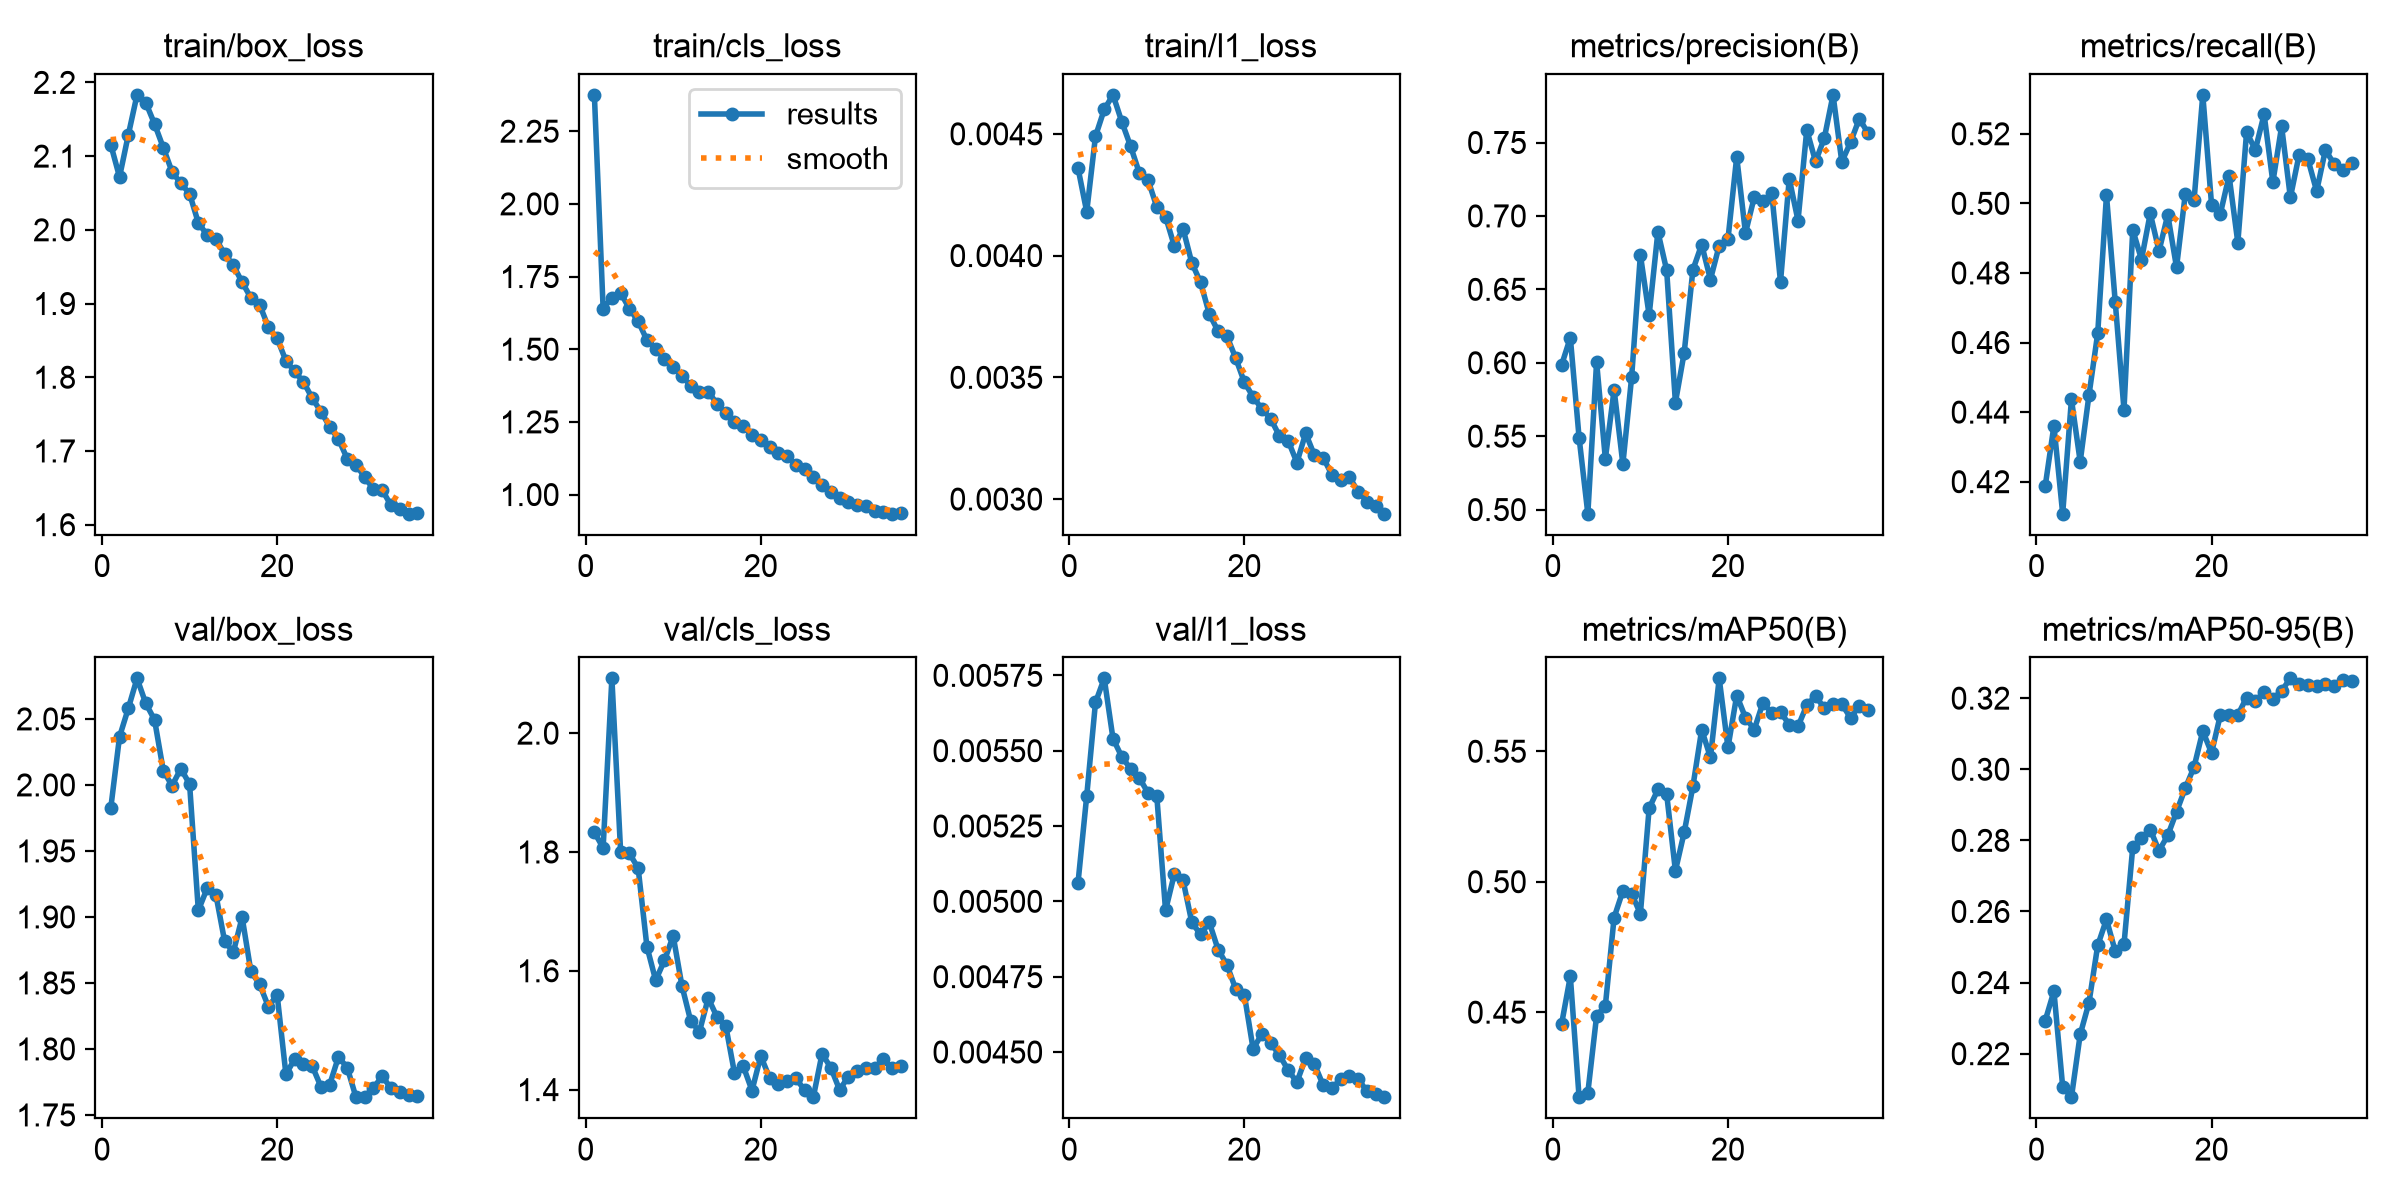
\includegraphics[width=0.9\linewidth]{ia/reel_results.png}
  \caption{Modèle d'anomalies routières (YOLO26s, 36 époques)}
\end{subfigure}

\vspace{0.2cm}
\begin{subfigure}[b]{\linewidth}\centering
  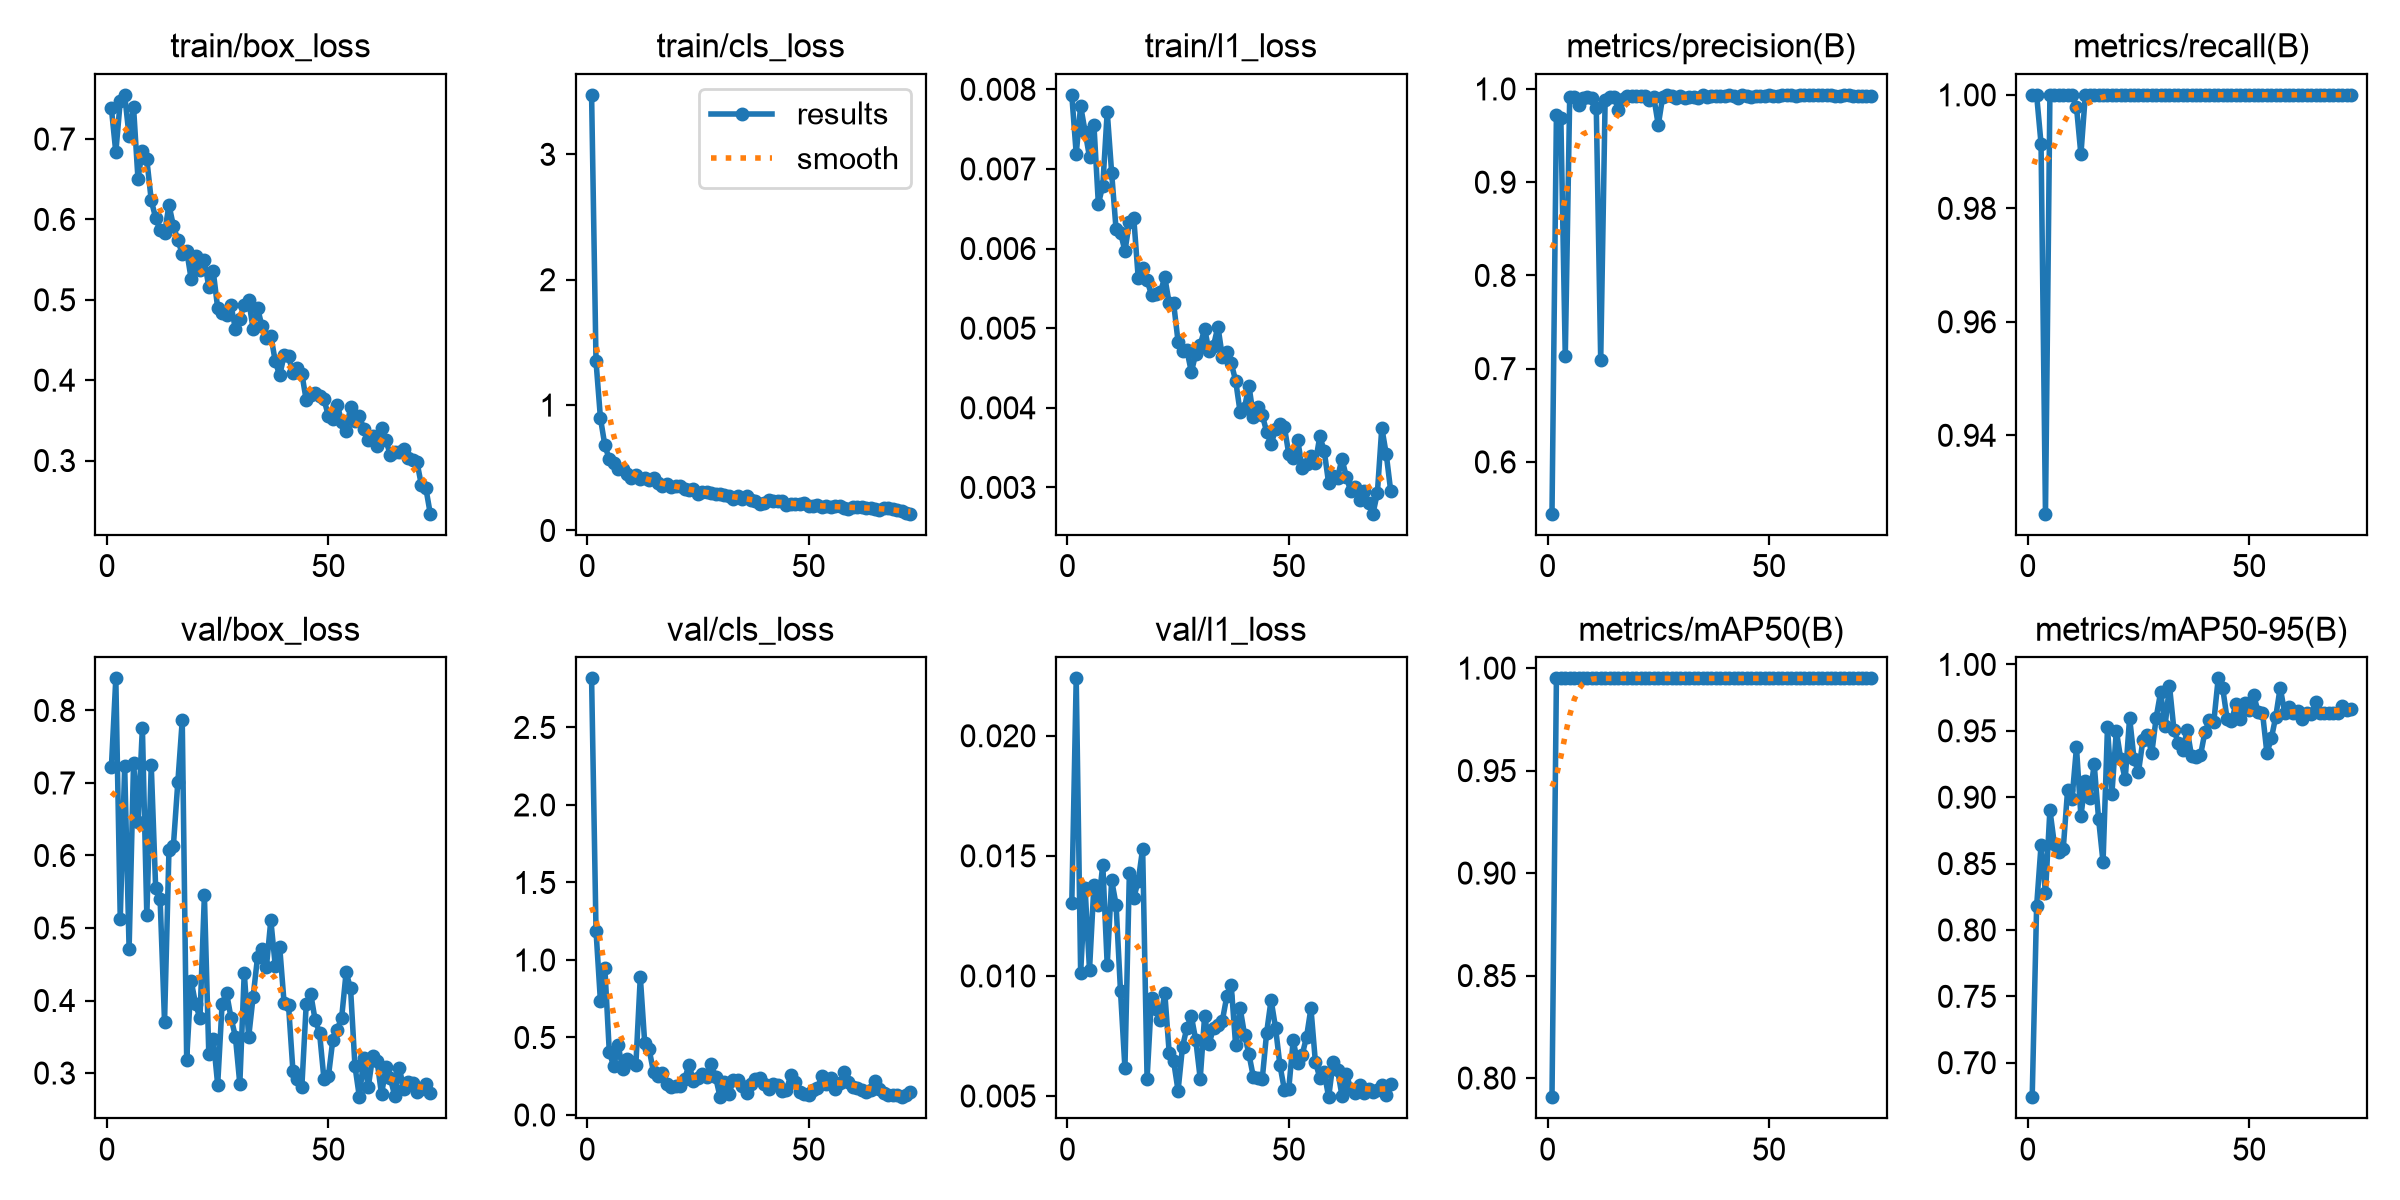
\includegraphics[width=0.9\linewidth]{ia/toy_results.png}
  \caption{Modèle du prototype (YOLO26n, 73 époques)}
\end{subfigure}
\caption{Courbes d'apprentissage : pertes d'entraînement et de validation, précision, rappel et mAP par époque}
\label{fig:courbes}
\end{figure}

\subsection{Sauvegarde et chargement des modèles}
À la fin de chaque notebook, les meilleurs poids sont exportés au format \textbf{ONNX} (\texttt{opset} 17,
graphe simplifié) et copiés dans le dossier \texttt{models/} de l'application, avec les poids PyTorch
(\texttt{.pt}) pour un éventuel réentraînement. Le notebook écrit aussi le profil du modèle et met à jour le
registre \texttt{models/registry.json}, qui contient les métriques d'évaluation affichées dans la page \emph{AI
models}. L'exemple suivant montre le profil du modèle du prototype :

\begin{lstlisting}[language=Python]
{ "name": "Toy track obstacles",
  "models": [ { "id": "toy-obstacles", "path": "models/toy_obstacles.onnx",
                "imgsz": 320, "conf": 0.4,
                "classes": { "column": "column", "box": "box" } } ] }
\end{lstlisting}

Au démarrage, l'application lit le profil de chaque environnement et charge les modèles avec ONNX Runtime ; un
modèle absent est simplement signalé (« pas encore entraîné ») sans empêcher l'application de fonctionner. Le format
ONNX rend l'application indépendante de PyTorch : elle n'a besoin que d'ONNX Runtime, beaucoup plus léger.

% =================================================================================================
\section{Détection et analyse des obstacles}

\subsection{Détection des objets et des anomalies routières}
Pour chaque image, le modèle renvoie une liste de détections : la classe de l'objet, un score de confiance et une
boîte englobante. En environnement réel, les deux modèles routiers analysent la même image et leurs détections
sont réunies.

\subsection{Localisation des objets dans les images}
La boîte indique où se trouve l'objet dans l'image. L'application en déduit deux informations simples :
\begin{itemize}
  \item \textbf{la distance} : plus un objet est proche, plus sa boîte est grande. Connaissant la taille habituelle
        de l'objet (environ 1,7 m pour un piéton, 0,7 m pour un cône), on estime sa distance à partir de la hauteur de
        sa boîte ; pour un nid-de-poule, objet plat, on utilise sa position dans l'image (plus il est bas, plus il est
        proche) ;
  \item \textbf{la position dans la voie} : l'obstacle est « sur la trajectoire » si sa boîte se trouve au centre de
        l'image, devant le véhicule, et « sur le côté » sinon.
\end{itemize}

\subsection{Exploitation des scores de confiance}
Le score de confiance, entre 0 et 1, indique la certitude du modèle. Les détections trop incertaines sont ignorées :
le seuil est de 0,40 pour les usagers de la route et pour le prototype, et de 0,35 pour les anomalies routières afin
de manquer moins de nids-de-poule. La confiance intervient aussi dans la gravité : une détection incertaine compte
moins qu'une détection certaine.

\subsection{Identification des nids-de-poule et des obstacles}
Les \textbf{anomalies fixes} (nid-de-poule, cône, barrière, panneau) sont enregistrées avec leur position sur la carte
et une photo. Les \textbf{usagers de la route} (piéton, cycliste, véhicule, animal) bougent : ils ne sont enregistrés
que s'ils sont devant le véhicule et proches. Un même obstacle vu plusieurs fois n'est enregistré qu'une seule fois,
avec un compteur d'observations. Enfin, un obstacle proche sur la trajectoire fait ralentir ou s'arrêter le véhicule.

\subsection{Estimation de la gravité des anomalies}
Chaque obstacle reçoit un score de gravité de 0 à 100, qui combine quatre éléments :
\begin{equation}
  \text{score} = 100 \times \underbrace{w}_{\text{danger de la classe}} \times
  \underbrace{(0{,}5 + 0{,}5\,p)}_{\text{proximité}} \times \underbrace{c}_{\text{confiance}} \times
  \underbrace{t}_{\text{trajectoire}}
\end{equation}
où $w$ est le poids de danger de la classe (1 pour un piéton, 0,6 pour un nid-de-poule, 0,4 pour un cône…), $p$ la
proximité entre 0 (loin) et 1 (très proche), $c$ la confiance du modèle et $t$ vaut 1 si l'obstacle est sur la
trajectoire et 0,5 s'il est sur le côté. Les poids de danger sont réglables dans l'application.

\subsection{Attribution d'un niveau de priorité}
Le score donne l'un des quatre niveaux de priorité du tableau~\ref{tab:niveaux}. Les obstacles sont ensuite triés du
plus grave au moins grave, pour que l'opérateur traite d'abord les plus dangereux.

\begin{table}[H]
\centering\small
\caption{Niveaux de priorité}
\label{tab:niveaux}
\begin{tabular}{l c l}
\toprule
\textbf{Niveau} & \textbf{Score} & \textbf{Signification} \\
\midrule
\textcolor{critique}{$\blacksquare$} Critique & $\geq 60$ & danger immédiat, à traiter en priorité \\
\textcolor{eleve}{$\blacksquare$} Élevé & 40 -- 60 & danger important \\
\textcolor{moyen}{$\blacksquare$} Moyen & 20 -- 40 & à surveiller \\
\textcolor{faible}{$\blacksquare$} Faible & $< 20$ & information \\
\bottomrule
\end{tabular}
\end{table}

Par exemple, un piéton proche ($p = 0{,}6$), détecté à 90\,\% sur la trajectoire, obtient
$100 \times 1 \times 0{,}8 \times 0{,}9 \times 1 = 72$ : il est \textbf{critique}. Un cône sur le côté, dans les mêmes
conditions, obtient $100 \times 0{,}4 \times 0{,}8 \times 0{,}9 \times 0{,}5 = 14{,}4$ : il est \textbf{faible}.

% =================================================================================================
\section{Évaluation des performances}

\subsection{Méthodologie d'évaluation}
Toutes les métriques finales sont mesurées sur les \textbf{ensembles de test}, jamais utilisés pendant l'entraînement
ni pour choisir les réglages. Pour le modèle routier, le réglage d'inférence (taille d'entrée, augmentation au
moment du test) a été choisi sur l'ensemble de validation, puis appliqué une seule fois au test. Nous indiquons
toujours le réglage correspondant à chaque résultat. Ultralytics donne la précision et le rappel au seuil de
confiance qui maximise le score F1 moyen ; les matrices de confusion sont calculées au seuil réellement utilisé dans
l'application.

\subsection{Précision, rappel et score F1}
Une détection est un \textbf{vrai positif} (TP) si elle correspond à un objet réel de la même classe, un
\textbf{faux positif} (FP) sinon ; un objet réel non détecté est un \textbf{faux négatif} (FN). On définit :
\begin{equation}
  \text{Précision} = \frac{TP}{TP + FP}, \qquad
  \text{Rappel} = \frac{TP}{TP + FN}, \qquad
  F_1 = 2 \cdot \frac{\text{Précision} \times \text{Rappel}}{\text{Précision} + \text{Rappel}}
\end{equation}
La précision mesure la fiabilité des alertes (peu de fausses alarmes), le rappel la capacité à ne pas manquer
d'obstacles. Pour un véhicule, un rappel élevé est souvent prioritaire, mais trop de fausses alarmes rendraient le
système inutilisable : le score F1 résume ce compromis.

\subsection{Intersection sur l'union (IoU) et mAP}
Pour décider si une boîte prédite correspond à un objet réel, on mesure leur recouvrement par l'\textbf{intersection
sur l'union} (figure~\ref{fig:iou}) :
\begin{equation} \text{IoU}(A, B) = \frac{|A \cap B|}{|A \cup B|} \end{equation}
Une prédiction est correcte si son IoU avec un objet réel dépasse un seuil (0,5 en général).

\begin{figure}[H]
\centering
\begin{tikzpicture}
  \fill[bleufst!25] (0,0) rectangle (2.4,1.8); \fill[orangefst!35] (1.2,0.6) rectangle (3.4,2.4);
  \fill[vertfst!70] (1.2,0.6) rectangle (2.4,1.8);
  \draw[thick,bleufst] (0,0) rectangle (2.4,1.8); \draw[thick,orangefst] (1.2,0.6) rectangle (3.4,2.4);
  \node[font=\scriptsize] at (0.55,0.3) {réelle}; \node[font=\scriptsize] at (2.95,2.15) {prédite};
  \node at (4.4,1.2) {$\text{IoU} = $};
  \begin{scope}[shift={(4.85,1.35)},scale=0.5]
    \fill[vertfst!70] (1.2,0.6) rectangle (2.4,1.8); \draw[thick,vertfst!60!black] (1.2,0.6) rectangle (2.4,1.8);
    \node[font=\scriptsize,anchor=west] at (3.6,1.2) {intersection};
  \end{scope}
  \draw[thick] (4.9,1.2) -- (6.7,1.2);
  \begin{scope}[shift={(4.95,-0.15)},scale=0.5]
    \fill[vertfst!40] (0,0) rectangle (2.4,1.8) (1.2,0.6) rectangle (3.4,2.4);
    \draw[thick,vertfst!60!black] (0,0) -- (2.4,0) -- (2.4,0.6) -- (3.4,0.6) -- (3.4,2.4) -- (1.2,2.4) -- (1.2,1.8)
                                  -- (0,1.8) -- cycle;
    \node[font=\scriptsize,anchor=west] at (3.6,1.2) {union};
  \end{scope}
\end{tikzpicture}
\caption{Intersection sur l'union entre une boîte réelle et une boîte prédite}
\label{fig:iou}
\end{figure}

En faisant varier le seuil de confiance, on obtient une courbe précision-rappel ; l'aire sous cette courbe est la
\textbf{précision moyenne} (AP) d'une classe. Le \textbf{mAP} est la moyenne des AP sur toutes les
classes~\cite{everingham2010voc,padilla2020metrics} :
\begin{itemize}
  \item \textbf{mAP@50} : IoU minimale de 0,5 ;
  \item \textbf{mAP@50-95} : moyenne des mAP pour des seuils d'IoU de 0,50 à 0,95 par pas de 0,05, plus exigeante
        sur la précision de localisation.
\end{itemize}

\subsection{Temps d'inférence et vitesse de traitement}
La vitesse est mesurée à deux niveaux (tableau~\ref{tab:vitesse}). Sur le GPU d'entraînement, Ultralytics mesure le
temps d'inférence pur par image. Dans l'application, les modèles ONNX s'exécutent sur le processeur de
l'ordinateur ; le temps dépend alors de la charge de la machine, car l'application, les simulateurs et le flux
vidéo partagent le même processeur.

\begin{table}[H]
\centering\small
\caption{Temps d'inférence mesurés}
\label{tab:vitesse}
\begin{tabularx}{\linewidth}{X l l}
\toprule
\textbf{Modèle et conditions} & \textbf{Temps par image} & \textbf{Cadence} \\
\midrule
Anomalies routières, GPU, 640 px & 10 ms & — \\
Anomalies routières, GPU, 960 px + TTA & 50 ms & — \\
Prototype, GPU, 320 px & 22 ms (30 ms en test ESP32) & — \\
Application, CPU : usagers + anomalies en parallèle (machine peu chargée) & $\approx$ 190 ms & $\approx$ 5 images/s \\
Application, CPU : usagers + anomalies (machine chargée) & $\approx$ 730 ms & $\approx$ 1,4 image/s \\
Application, CPU : modèle du prototype (image 480\,$\times$\,640) & $\approx$ 70 ms & $\approx$ 14 images/s \\
\bottomrule
\end{tabularx}
\end{table}

\subsection{Résultats obtenus sur les données réelles}\label{sec:resultats-reels}
Le tableau~\ref{tab:res-reel} donne les résultats du détecteur d'anomalies routières sur les 815 images de test
(5\,105 objets), au réglage temps réel utilisé dans l'application (640 px) et au meilleur réglage hors ligne
(960 px avec augmentation au moment du test, TTA).

\begin{table}[H]
\centering\small
\caption{Résultats du détecteur d'anomalies routières sur l'ensemble de test}
\label{tab:res-reel}
\begin{tabular}{l r cccc c cccc}
\toprule
 & & \multicolumn{4}{c}{\textbf{640 px (temps réel)}} & & \multicolumn{4}{c}{\textbf{960 px + TTA}} \\
\cmidrule{3-6}\cmidrule{8-11}
\textbf{Classe} & \textbf{Objets} & P & R & mAP50 & mAP50-95 & & P & R & mAP50 & mAP50-95 \\
\midrule
nid-de-poule & 299  & 0,601 & 0,254 & 0,312 & 0,108 & & 0,626 & 0,268 & 0,330 & 0,119 \\
cône         & 2\,358 & 0,712 & 0,715 & 0,694 & 0,416 & & 0,681 & 0,763 & 0,744 & 0,464 \\
barrière     & 1\,977 & 0,692 & 0,539 & 0,578 & 0,317 & & 0,688 & 0,594 & 0,634 & 0,369 \\
panneau      & 471  & 0,638 & 0,495 & 0,520 & 0,367 & & 0,630 & 0,567 & 0,588 & 0,430 \\
\midrule
\textbf{toutes} & \textbf{5\,105} & \textbf{0,661} & \textbf{0,501} & \textbf{0,526} & \textbf{0,302} & &
  \textbf{0,656} & \textbf{0,548} & \textbf{0,574} & \textbf{0,346} \\
\bottomrule
\end{tabular}
\end{table}

Les cônes et les barrières, nombreux et bien contrastés, sont les mieux reconnus. Les nids-de-poule restent
difficiles (AP@50 de 0,31) : ils sont peu nombreux dans l'ensemble (299 objets de test) et visuellement très
variables. Le réglage 960 px + TTA améliore le mAP@50 de 0,526 à 0,574, au prix d'un temps d'inférence cinq fois
plus long ; il n'est donc pas utilisé en temps réel.

Deux analyses complémentaires éclairent ces chiffres. D'une part, si l'on ne demande au modèle que de \emph{trouver}
l'obstacle sans en nommer le type exact (évaluation agnostique de la classe, un cône pris pour une barrière restant
une détection correcte), le mAP@50 atteint 0,630 en temps réel et 0,677 au meilleur réglage
(tableau~\ref{tab:agnostique}). D'autre part, le seuil de confiance règle le compromis entre fausses alarmes et
obstacles manqués : à un seuil de 0,70, la précision moyenne atteint 0,916, mais le rappel tombe à 0,300.

\begin{table}[H]
\centering\small
\caption{Évaluation agnostique de la classe et points de fonctionnement (ensemble de test)}
\label{tab:agnostique}
\begin{tabular}{lccccc}
\toprule
\textbf{Évaluation agnostique} & P & R & F1 & mAP50 & mAP50-95 \\
\midrule
640 px (temps réel) & 0,726 & 0,597 & 0,655 & 0,630 & 0,364 \\
960 px + TTA & 0,711 & 0,646 & 0,677 & 0,677 & 0,412 \\
\bottomrule
\end{tabular}

\vspace{0.3cm}
\begin{tabular}{ccccc}
\toprule
\textbf{Seuil de confiance} & \textbf{P (par classe)} & \textbf{R (par classe)} & \textbf{P (agnostique)} &
\textbf{R (agnostique)} \\
\midrule
0,25 & 0,520 & 0,612 & 0,563 & 0,720 \\
0,40 & 0,673 & 0,534 & 0,707 & 0,647 \\
0,50 & 0,763 & 0,474 & 0,781 & 0,579 \\
0,70 & 0,916 & 0,300 & 0,893 & 0,370 \\
\bottomrule
\end{tabular}
\end{table}

La figure~\ref{fig:courbes-reel} présente les courbes précision-rappel et F1 ainsi que la matrice de confusion au
seuil utilisé dans l'application (0,35). La matrice montre que les confusions entre classes sont rares (au plus
3\,\%) : les erreurs sont surtout des objets manqués (ligne \emph{background}) et des fausses détections sur le
fond, en particulier des cônes.

\begin{figure}[H]
\centering
\begin{subfigure}[b]{0.49\linewidth}\centering
  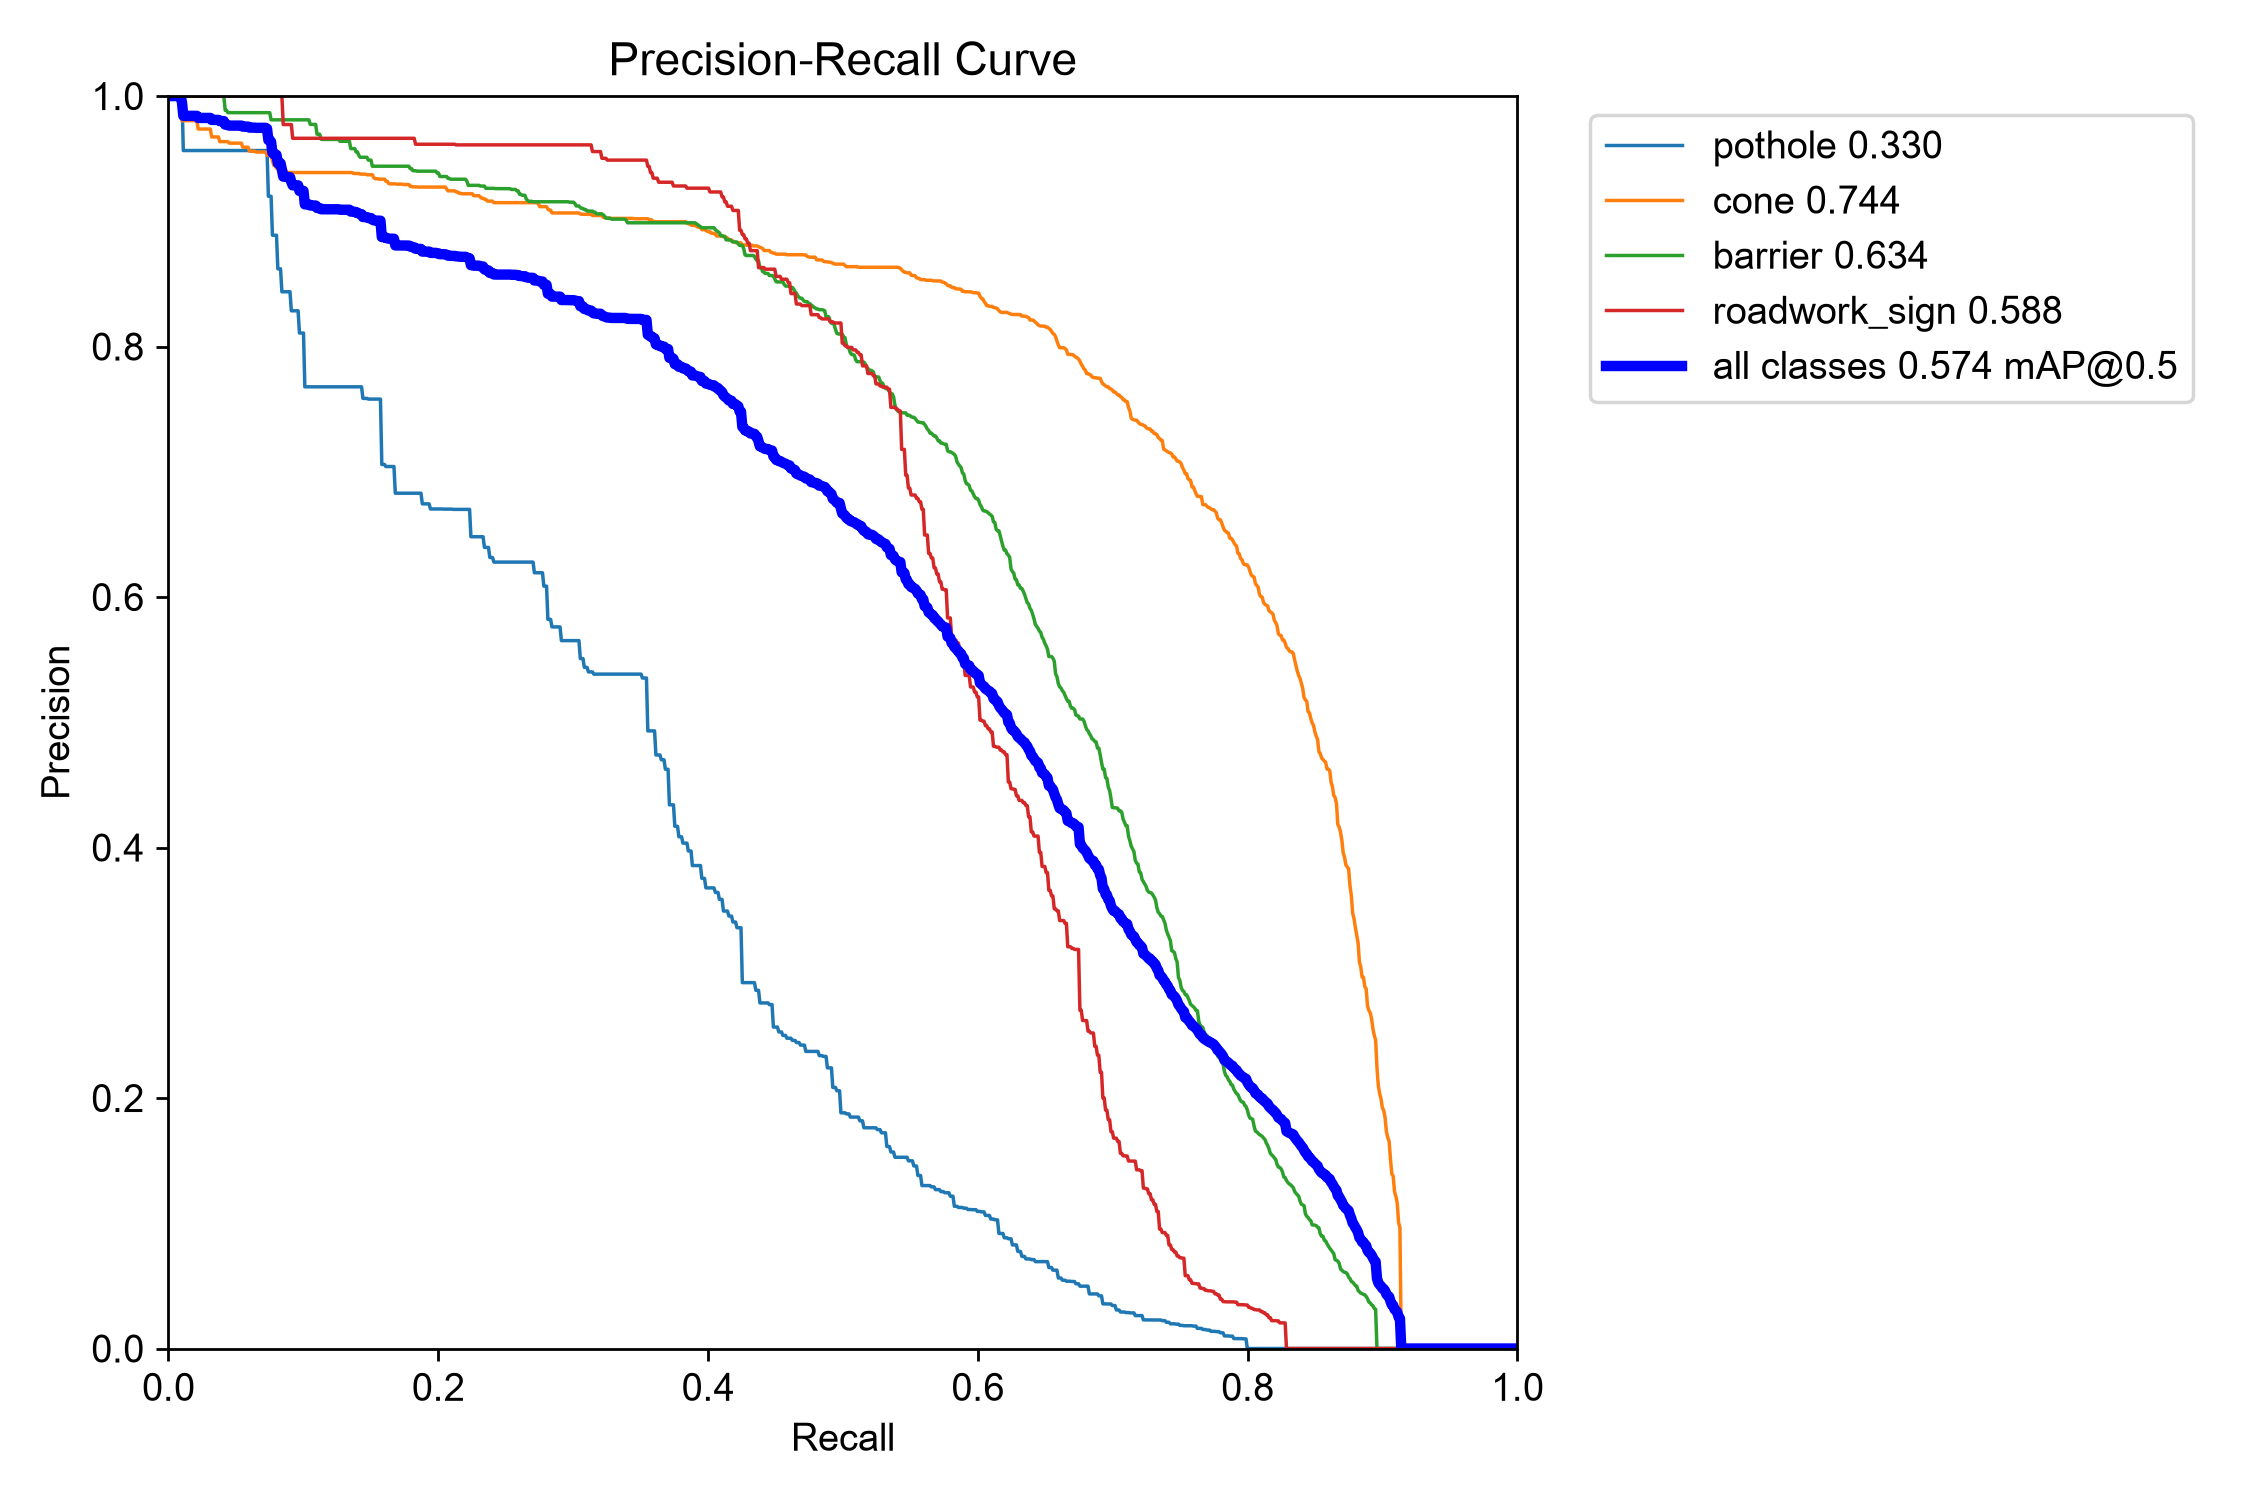
\includegraphics[width=\linewidth]{ia/reel_pr.png}
  \caption{Courbes précision-rappel (960 px + TTA)}
\end{subfigure}\hfill
\begin{subfigure}[b]{0.49\linewidth}\centering
  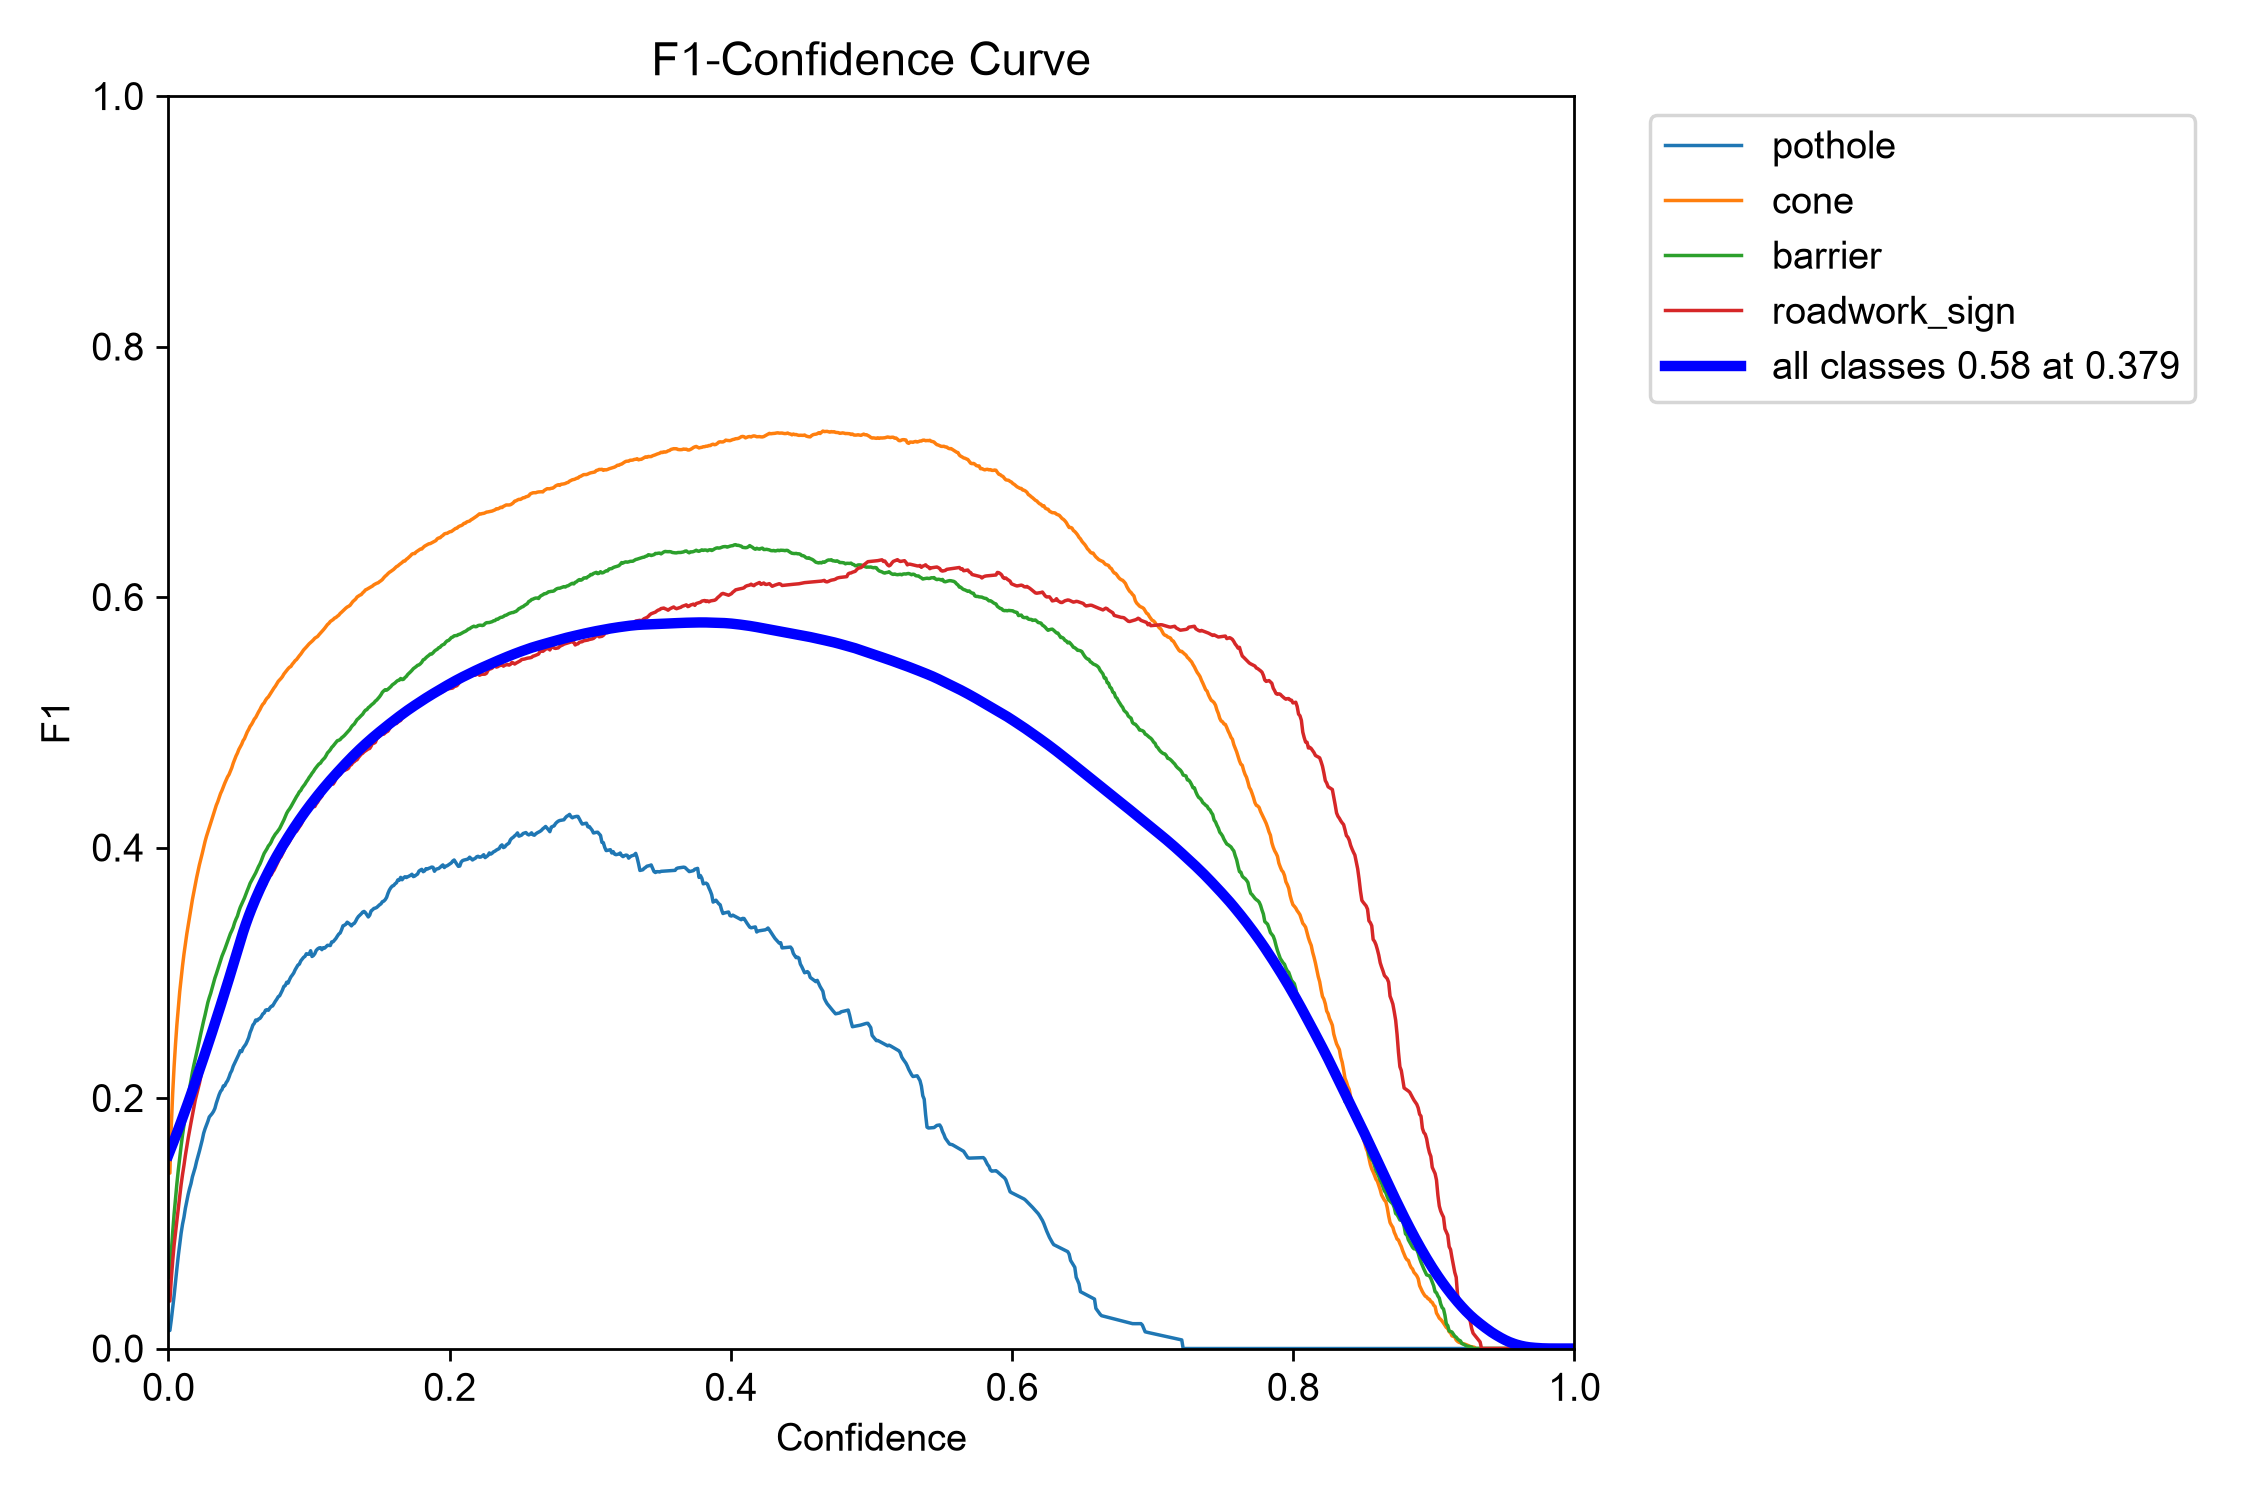
\includegraphics[width=\linewidth]{ia/reel_f1.png}
  \caption{Score F1 en fonction du seuil}
\end{subfigure}

\vspace{0.2cm}
\begin{subfigure}[b]{0.62\linewidth}\centering
  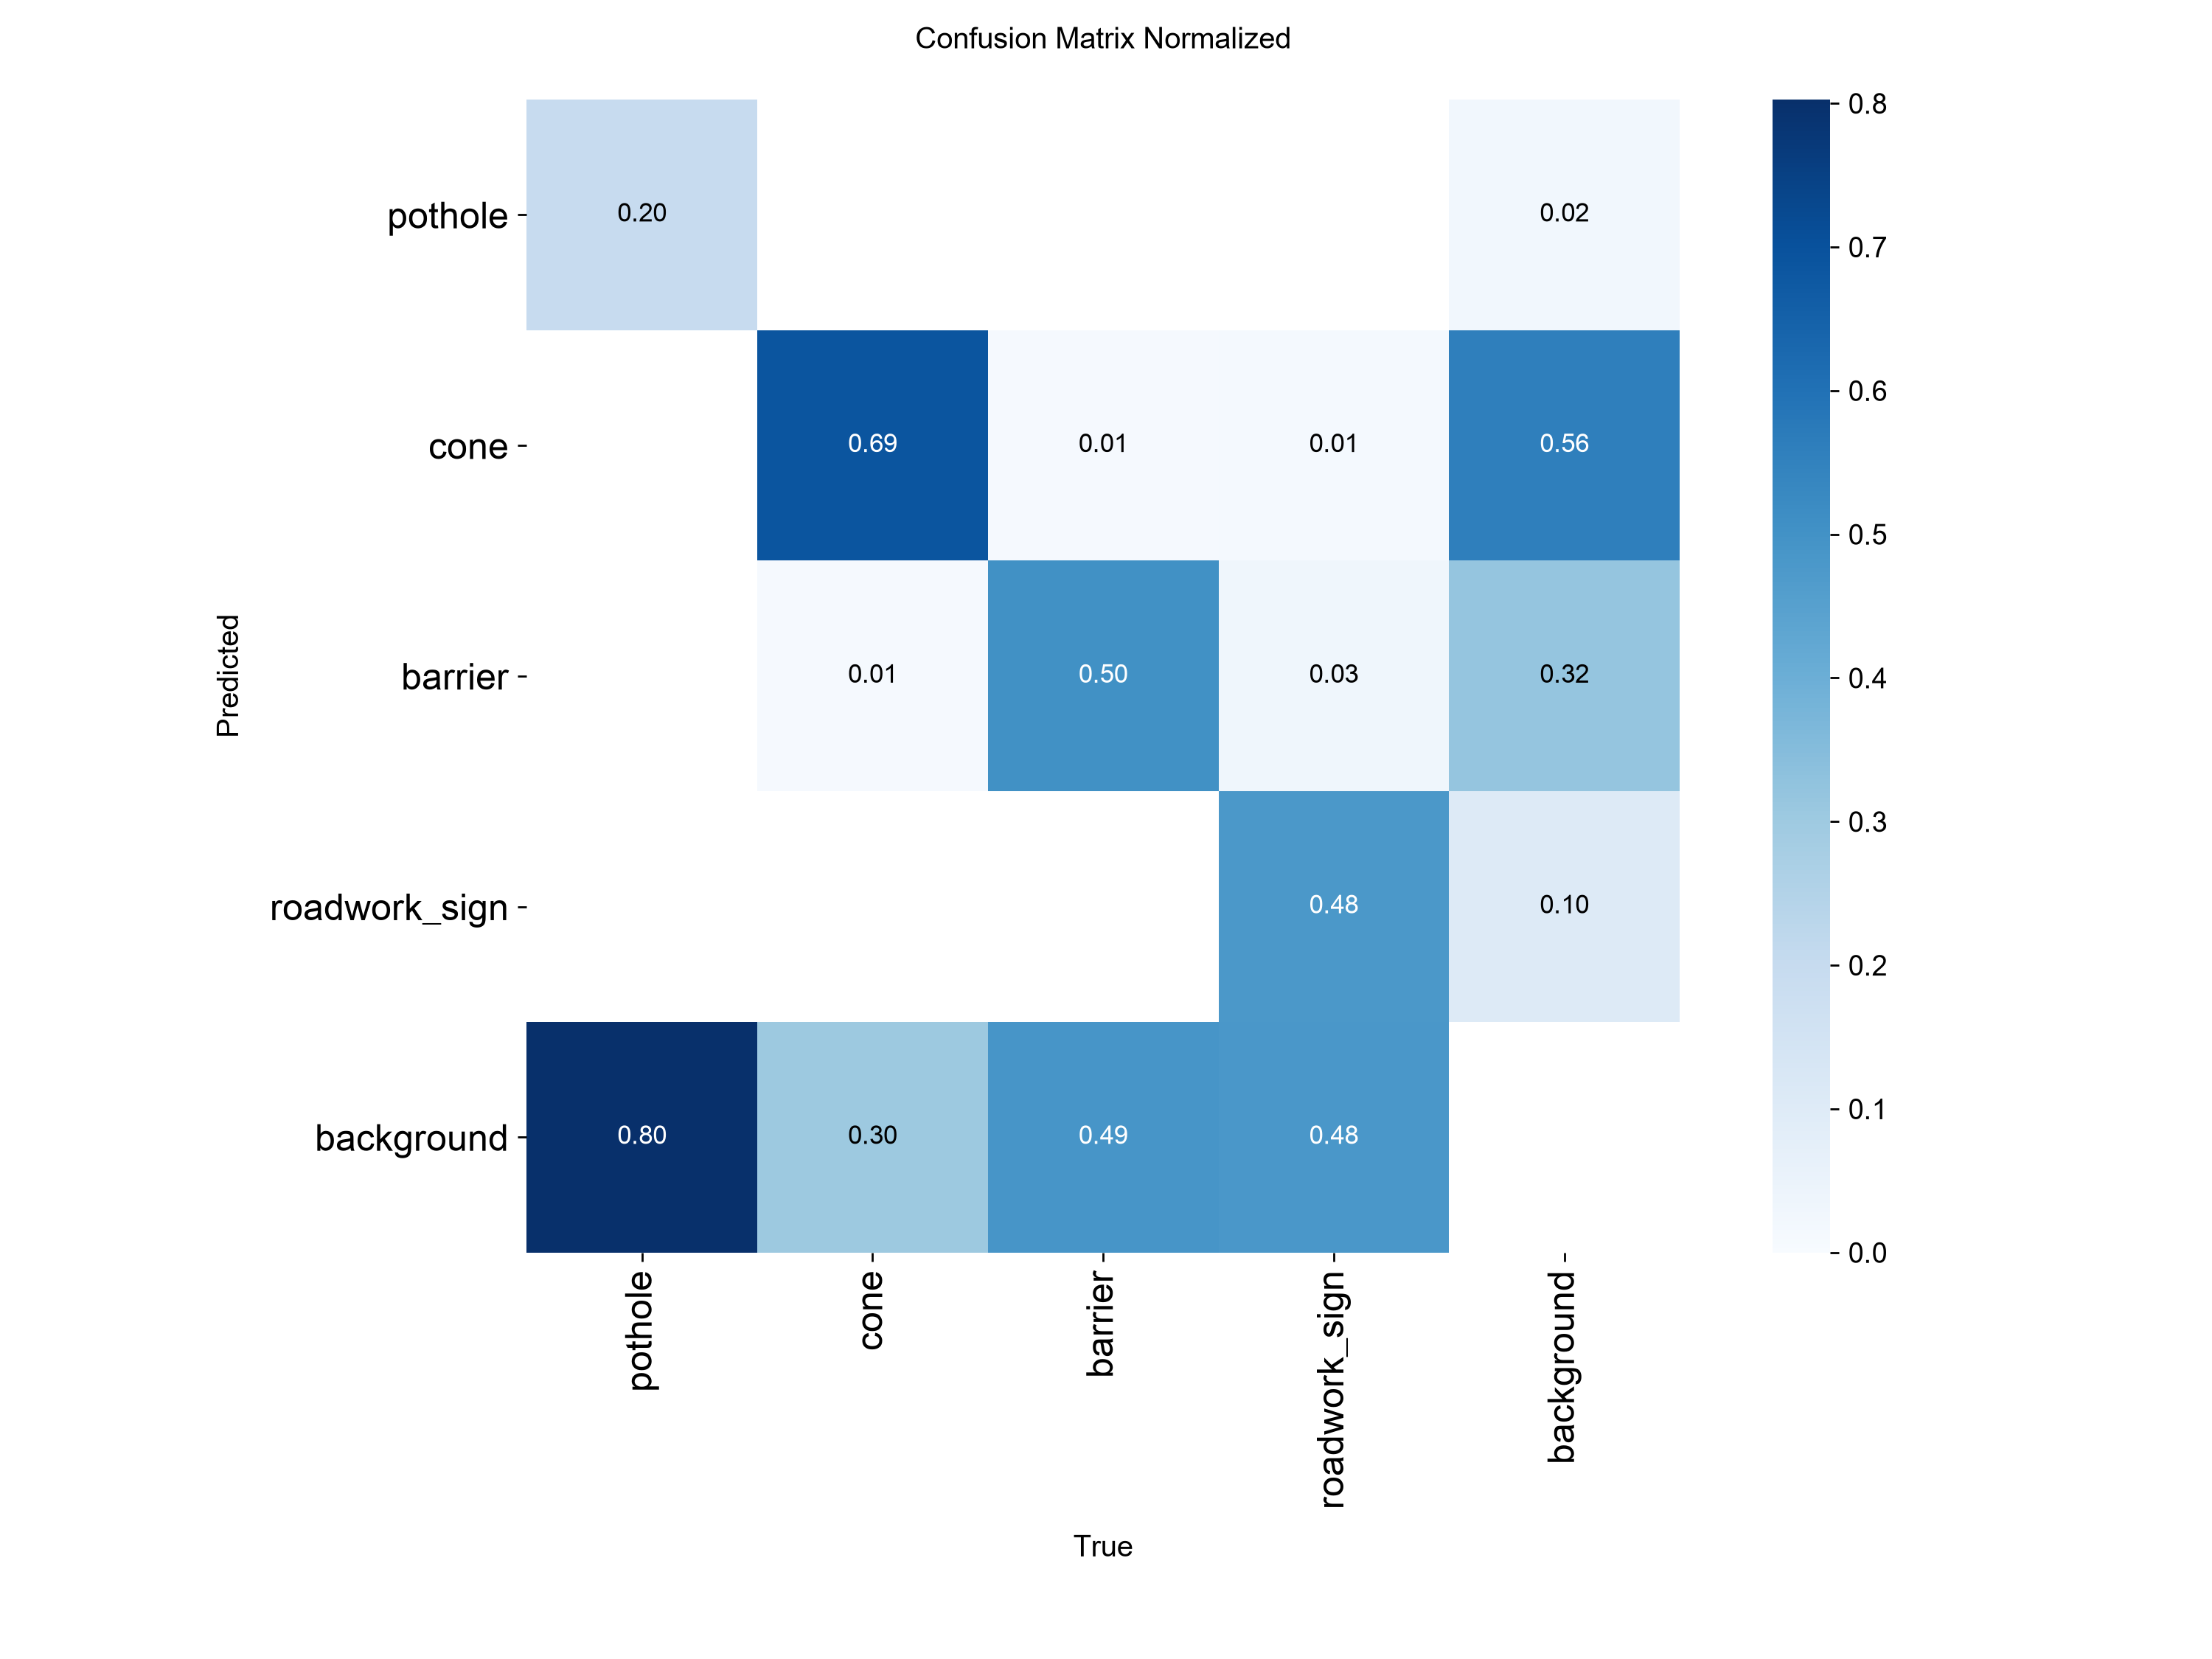
\includegraphics[width=\linewidth]{ia/reel_confusion.png}
  \caption{Matrice de confusion normalisée (640 px, seuil 0,35)}
\end{subfigure}
\caption{Résultats du détecteur d'anomalies routières sur l'ensemble de test}
\label{fig:courbes-reel}
\end{figure}

\subsection{Résultats obtenus sur les données du prototype}
Le tableau~\ref{tab:res-proto} donne les résultats du modèle du prototype sur ses deux ensembles de test. Au seuil
de 0,40 utilisé dans l'application, les 15 obstacles des images de test sont tous détectés avec la bonne classe,
sans aucune fausse détection, aussi bien sur les images d'origine que sur leurs versions au style ESP32-CAM
(tableau~\ref{tab:conf-proto}). Le mAP@50-95 plus faible sur les images ESP32-CAM (0,921 contre 0,976) traduit des
boîtes un peu moins précises sur des images petites et dégradées.

\begin{table}[H]
\centering\small
\caption{Résultats du modèle du prototype sur l'ensemble de test (26 images, 15 obstacles)}
\label{tab:res-proto}
\begin{tabular}{lccccc}
\toprule
\textbf{Ensemble de test} & P & R & F1 & mAP50 & mAP50-95 \\
\midrule
Images d'origine (832\,$\times$\,464) & 0,989 & 1,000 & 0,994 & 0,995 & 0,976 \\
Mêmes images au style ESP32-CAM (320\,$\times$\,240) & 0,991 & 1,000 & 0,995 & 0,995 & 0,921 \\
\bottomrule
\end{tabular}
\end{table}

\begin{table}[H]
\centering\small
\caption{Matrice de confusion du modèle du prototype (test, seuil 0,40)}
\label{tab:conf-proto}
\begin{tabular}{l|ccc}
\toprule
\textbf{Réel $\backslash$ prédit} & \textbf{colonne} & \textbf{boîte} & \textbf{fond (manqué)} \\
\midrule
colonne & 6 & 0 & 0 \\
boîte & 0 & 9 & 0 \\
fond (fausse détection) & 0 & 0 & — \\
\bottomrule
\end{tabular}
\end{table}

\begin{figure}[H]
\centering
\begin{subfigure}[b]{0.49\linewidth}\centering
  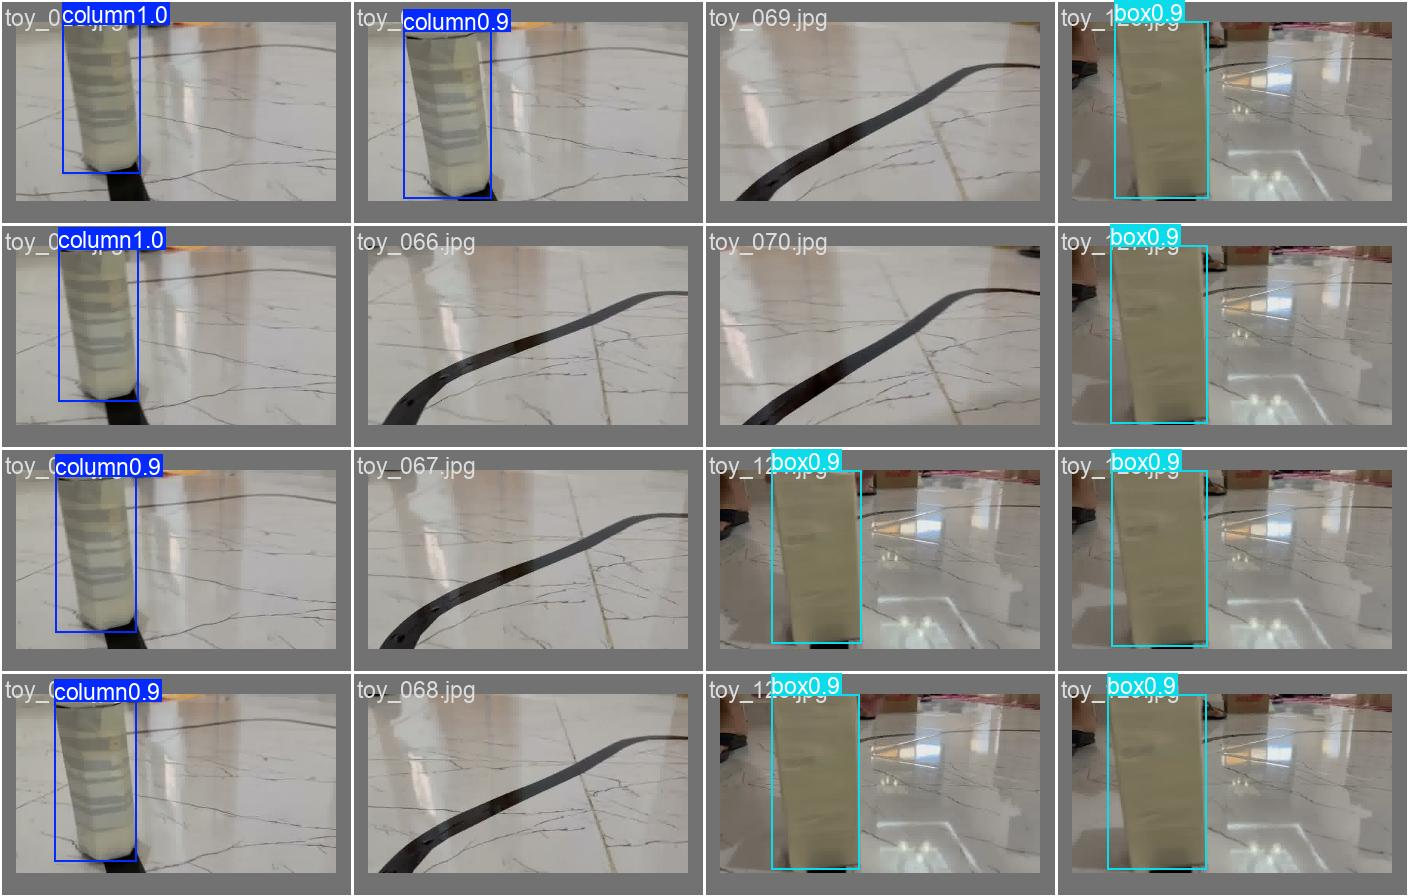
\includegraphics[width=\linewidth]{ia/toy_test_pred.jpg}
  \caption{Images de test d'origine}
\end{subfigure}\hfill
\begin{subfigure}[b]{0.49\linewidth}\centering
  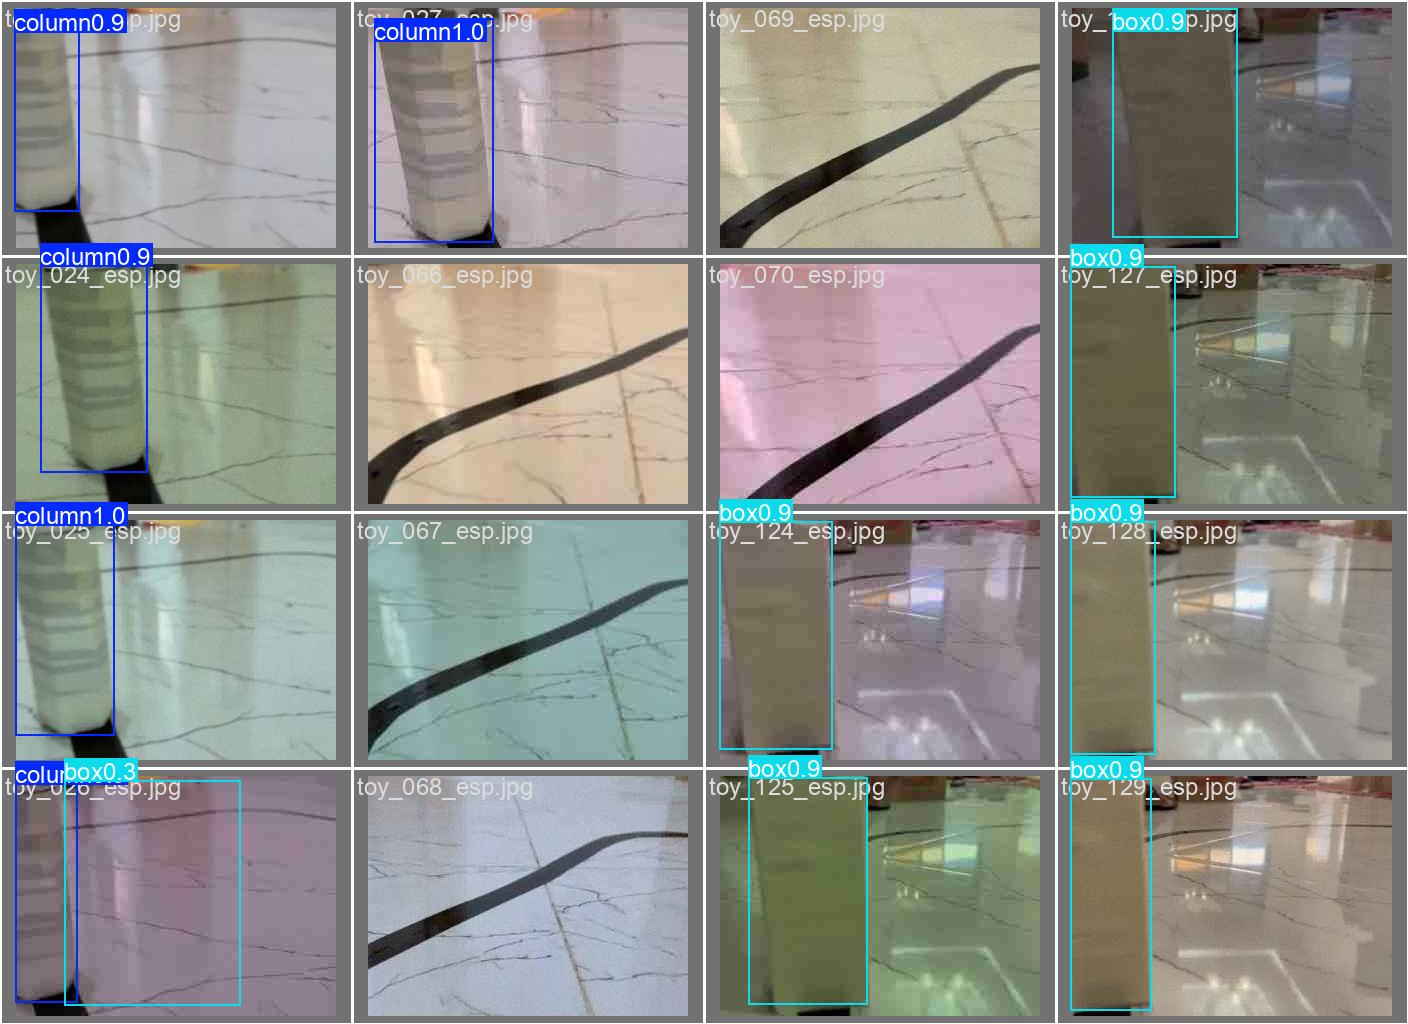
\includegraphics[width=\linewidth]{ia/toy_test_esp32_pred.jpg}
  \caption{Images de test au style ESP32-CAM}
\end{subfigure}

\vspace{0.2cm}
\begin{subfigure}[b]{0.49\linewidth}\centering
  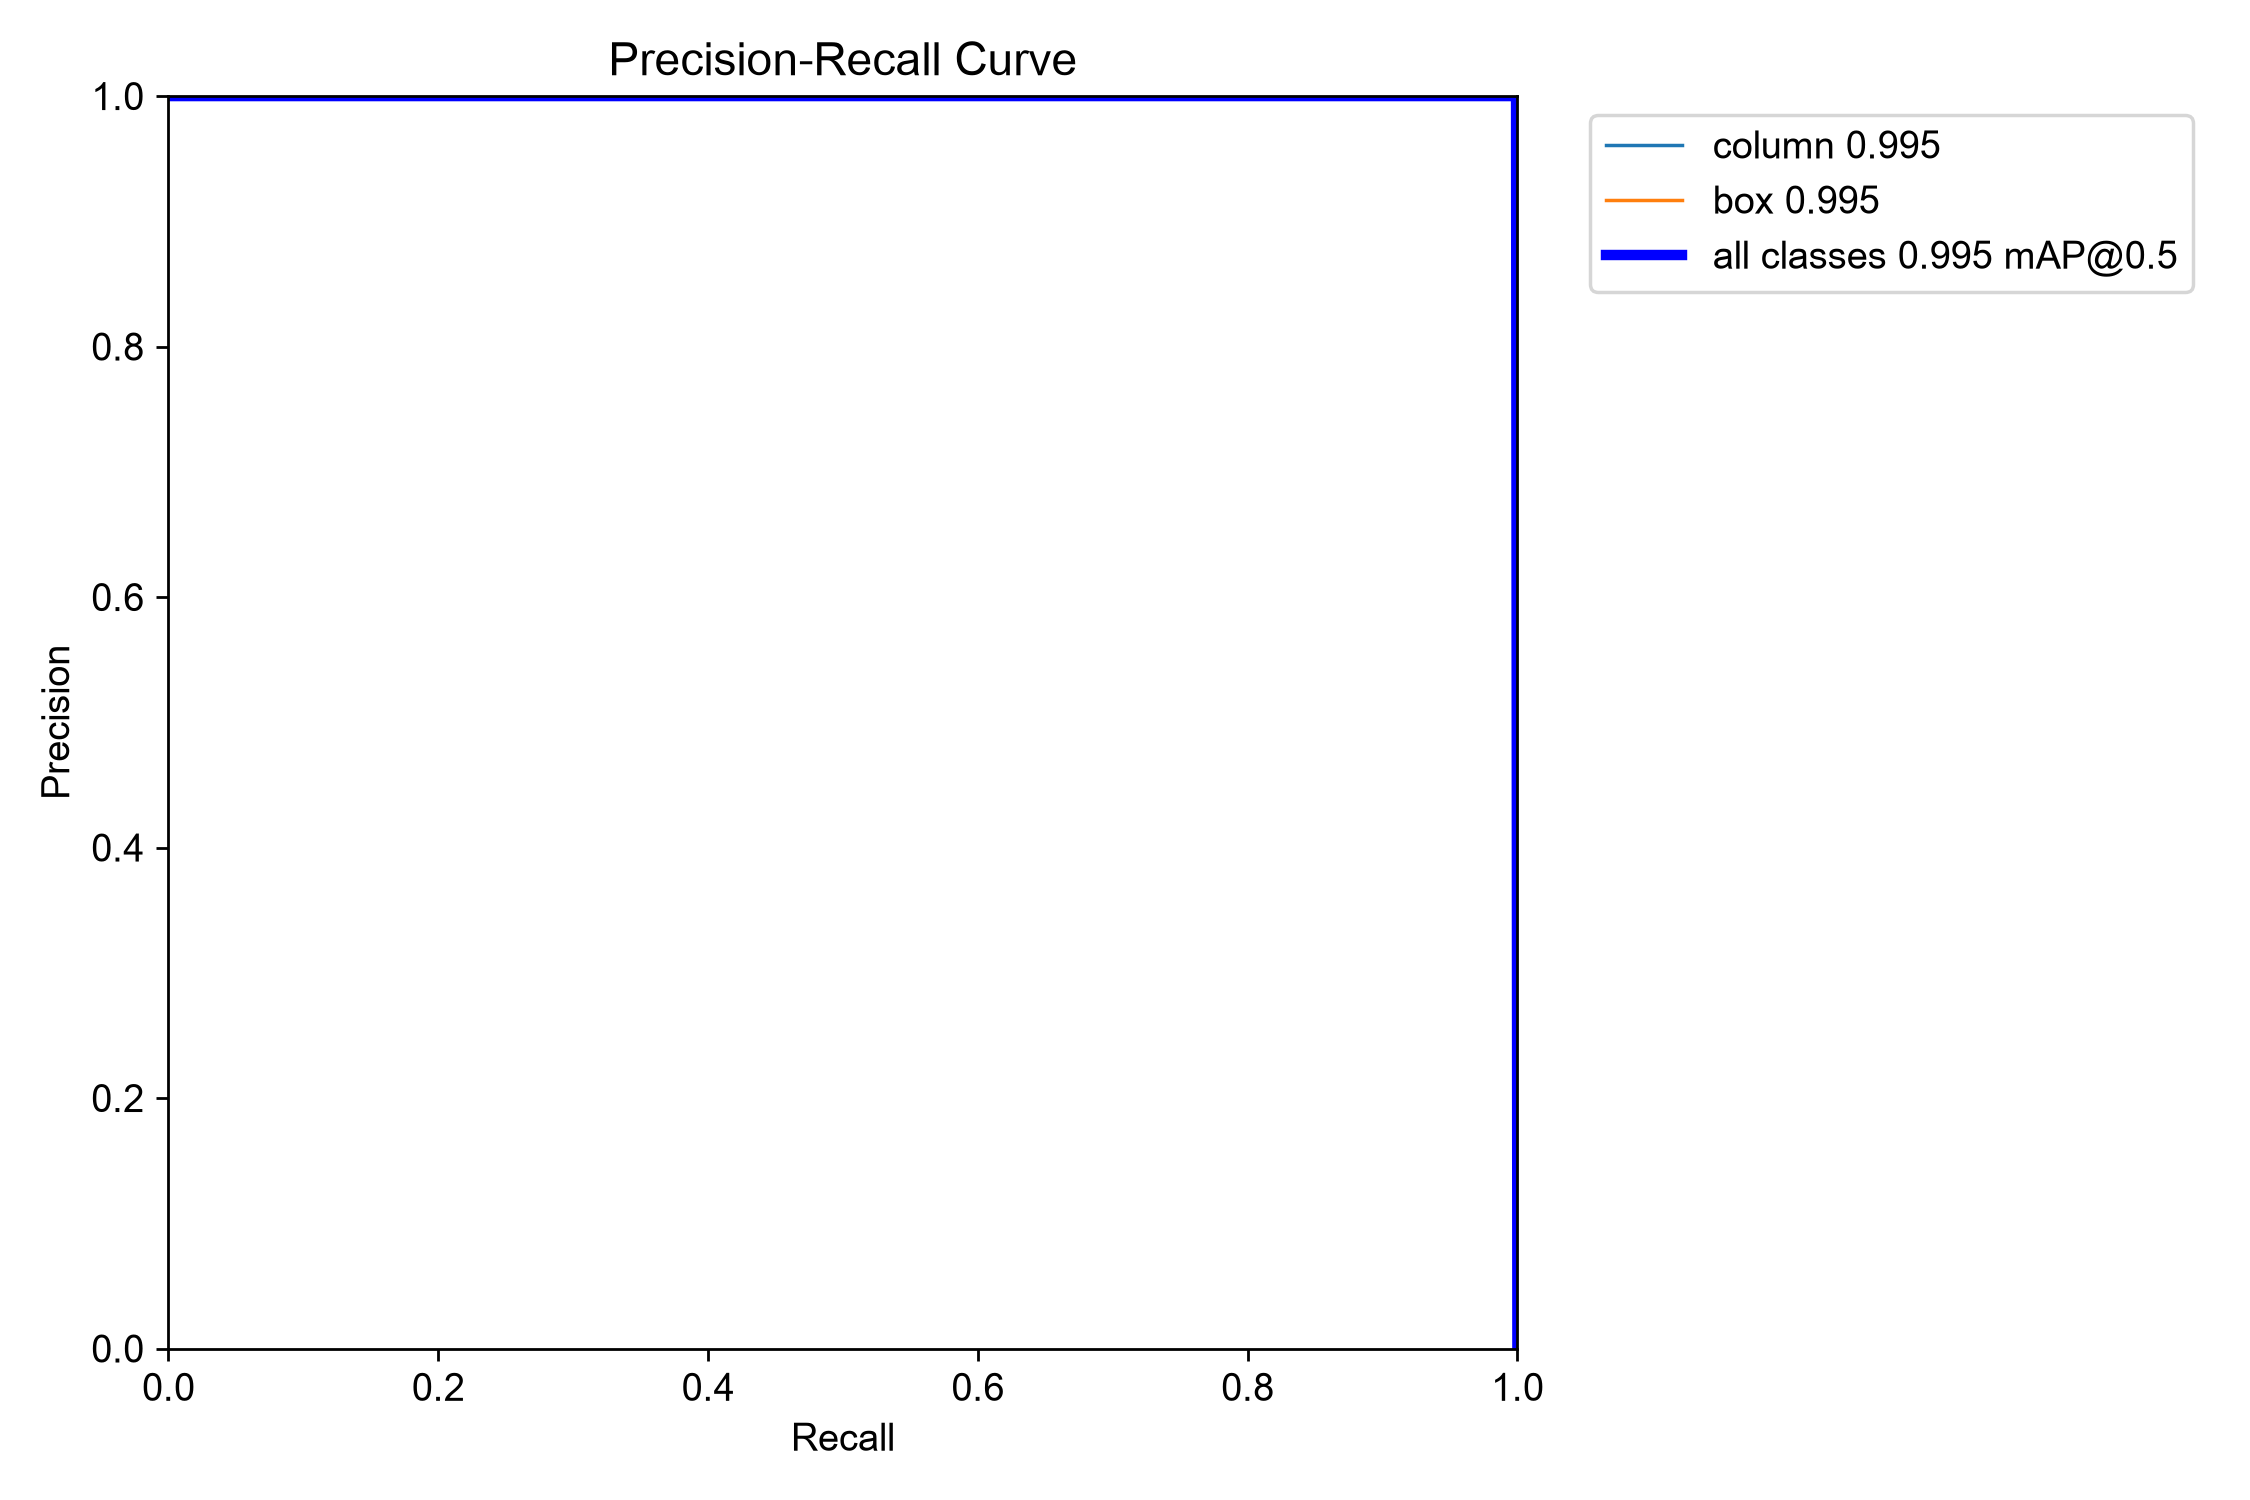
\includegraphics[width=\linewidth]{ia/toy_pr.png}
  \caption{Courbe précision-rappel}
\end{subfigure}\hfill
\begin{subfigure}[b]{0.49\linewidth}\centering
  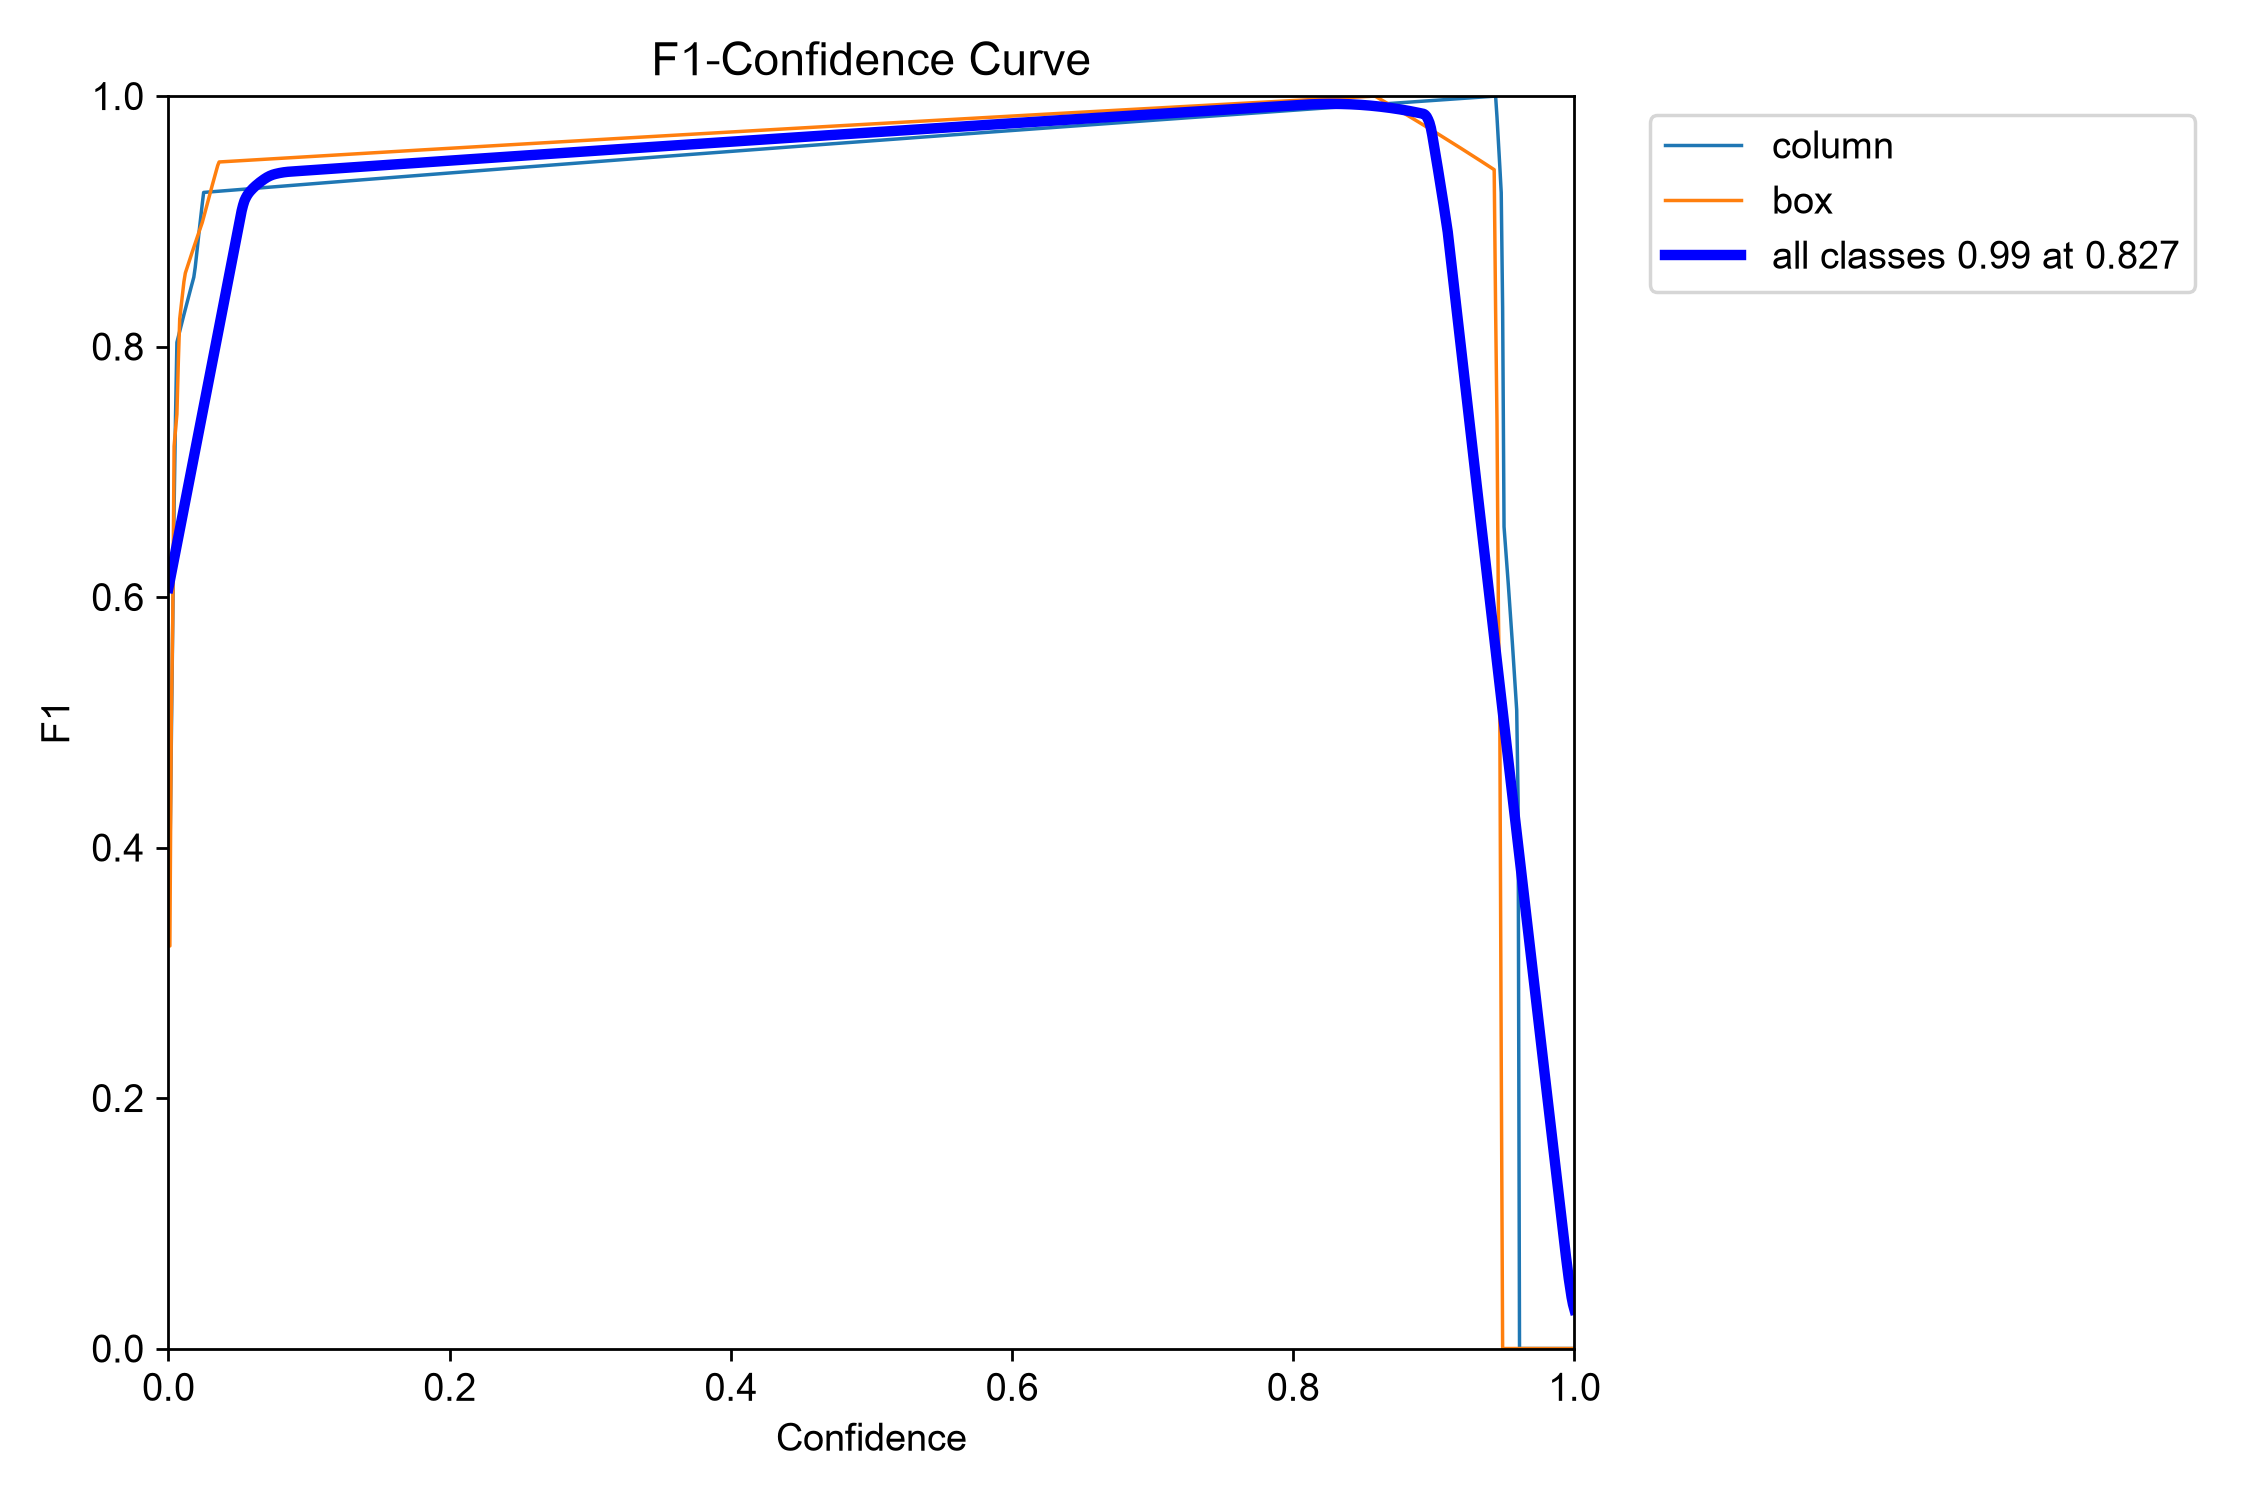
\includegraphics[width=\linewidth]{ia/toy_f1.png}
  \caption{Score F1 en fonction du seuil}
\end{subfigure}
\caption{Résultats du modèle du prototype sur l'ensemble de test}
\label{fig:res-proto}
\end{figure}

Ces résultats doivent être nuancés. L'ensemble de test est petit et provient de la même vidéo que l'entraînement
(même éclairage, même sol), même si le découpage temporel évite les quasi-doublons. Le test sur la vraie caméra
de la voiture, réalisé après l'entraînement, confirme que la boîte est reconnue avec une confiance de 95\,\%
(figure~\ref{fig:test-reel-proto}) ; il a aussi révélé deux limites. D'une part, la caméra étant montée sur la
tranche, l'image doit être redressée avant l'analyse : sans rotation, le modèle ne détecte rien. D'autre part, des
éléments jamais vus pendant l'entraînement, comme un meuble brun en bord d'image ou une main devant l'objectif,
ont parfois été pris pour une colonne. L'enregistrement d'images réelles de l'ESP32-CAM, prévu dans l'application,
permettra d'ajouter ces cas à l'entraînement.

\begin{figure}[H]
\centering
\begin{subfigure}[b]{0.52\linewidth}\centering
  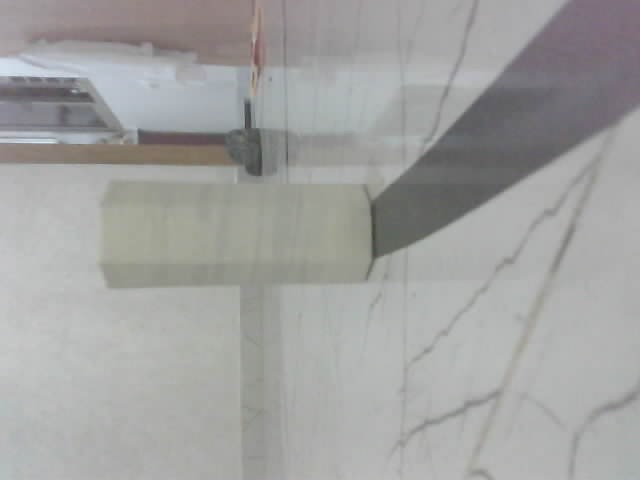
\includegraphics[height=4.6cm]{captures/esp32_brut_tourne.jpg}
  \caption{Image brute (caméra sur la tranche) : aucune détection}
\end{subfigure}\hfill
\begin{subfigure}[b]{0.44\linewidth}\centering
  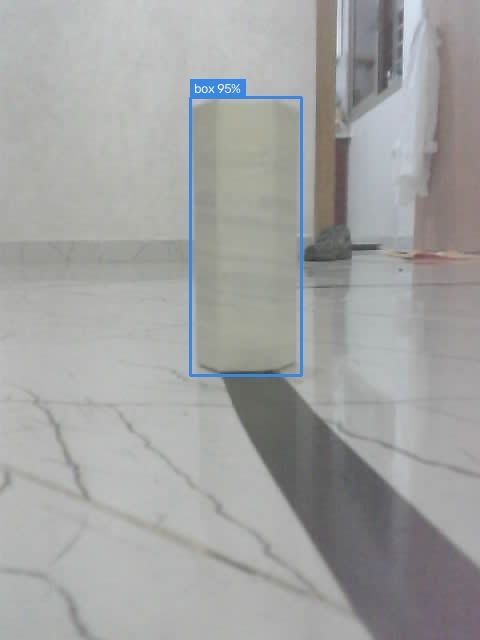
\includegraphics[height=4.6cm]{captures/esp32_detection_box.jpg}
  \caption{Image redressée : boîte détectée à 95\,\%}
\end{subfigure}
\caption{Test du modèle du prototype sur le flux réel de l'ESP32-CAM}
\label{fig:test-reel-proto}
\end{figure}

\subsection{Analyse comparative des deux modèles}
Le tableau~\ref{tab:comparaison} compare les deux modèles entraînés. L'écart de performances s'explique d'abord par
la difficulté des tâches : le modèle routier doit reconnaître des objets très variés dans des milliers de scènes
différentes (villes, météo, éclairage), alors que le modèle du prototype reconnaît deux objets bien définis dans un
environnement contrôlé. Les résultats du modèle routier, obtenus sur des lieux absents de l'entraînement, sont donc
plus représentatifs d'un usage réel ; ceux du prototype mesurent surtout la bonne adaptation au circuit.

\begin{table}[H]
\centering\small
\caption{Comparaison des deux modèles entraînés}
\label{tab:comparaison}
\begin{tabularx}{\linewidth}{l X X}
\toprule
\textbf{Critère} & \textbf{Anomalies routières} & \textbf{Prototype} \\
\midrule
Variante & YOLO26s (\emph{small}) & YOLO26n (\emph{nano}) \\
Données & 7\,894 images réelles, 4 classes & 249 images d'une vidéo + augmentations, 2 classes \\
Entraînement & 8 h, 36 époques & 30 min, 73 époques \\
mAP@50 (test) & 0,526 (temps réel), 0,574 (meilleur réglage) & 0,995 \\
mAP@50-95 (test) & 0,302, 0,346 & 0,976 (0,921 style ESP32) \\
Vitesse sur CPU & 1,4 à 5 images/s (avec le modèle des usagers) & $\approx$ 14 images/s \\
Point fort & généralisation à des lieux inconnus & très fiable sur son circuit \\
Limite & nids-de-poule (rappel 0,25) & domaine étroit, petit test \\
\bottomrule
\end{tabularx}
\end{table}

\chapconclusion
Ce chapitre a présenté la conception des modèles de détection : le choix de YOLO26, la constitution et l'annotation
des données (dont une annotation automatique par SAM~2 pour le prototype), l'entraînement dans un environnement
Docker reproductible, l'exploitation des détections (distance, gravité, priorité) et une évaluation détaillée. Le
modèle routier atteint un mAP@50 de 0,53 en temps réel sur des lieux inconnus, et le modèle du prototype reconnaît
tous les obstacles de son ensemble de test. Le chapitre suivant présente l'application qui exploite ces modèles.
